% Rewritten from the user-designated ARR PDF, 12 September 2026.
% Official ICLR 2027 style files are included without modification.
% Compile with pdflatex -no-shell-escape, bibtex, then pdflatex twice.
\documentclass{article}
\PassOptionsToPackage{sort}{natbib}
\usepackage{iclr2027_conference,times}
% Numeric references in order of first citation, as requested by the author.
\setcitestyle{numbers,square,citesep={,}}
\usepackage[T1]{fontenc}
\usepackage[utf8]{inputenc}
\usepackage{microtype,amsmath,amssymb,booktabs,graphicx,multirow}
\usepackage{enumitem,tabularx,array,flafter,placeins}
\usepackage[table]{xcolor}
\definecolor{resultshade}{gray}{0.94}
\definecolor{paperlink}{RGB}{0,70,145}
\usepackage{hyperref,url}
\hypersetup{colorlinks=true,linkcolor=paperlink,citecolor=paperlink,urlcolor=paperlink,
  pdfborder={0 0 0},pdftitle={CoMem: Reusing Transformer Depth across Queries},pdfauthor={Anonymous}}
\newcommand{\writepass}{\textsc{Write}}
\newcommand{\selectpass}{\textsc{Select}}
\newcommand{\readpass}{\textsc{Read}}
\newcommand{\comem}{CoMem}
\newcolumntype{Y}{>{\raggedright\arraybackslash}X}
\renewcommand{\topfraction}{0.9}
\renewcommand{\bottomfraction}{0.8}
\renewcommand{\textfraction}{0.08}
\renewcommand{\floatpagefraction}{0.75}
\setcounter{topnumber}{3}
\setcounter{totalnumber}{4}
\title{CoMem: Reusing Transformer Depth across Queries}
\author{Anonymous authors\\Paper under double-blind review}
% \iclrfinalcopy
\begin{document}
\maketitle
\begin{abstract}
Early transformer layers map document tokens into intermediate semantic representations that later layers can use for prediction. Our key insight is to reuse this encoder-like computation across queries by placing a persistent cache between the two parts of the decoder. CoMem (Comprehension Memory) treats the lower layers as a semantic encoder and the remaining layers as a reader. Write encodes document chunks once and stores their intermediate residuals; Read retrieves selected cached states, combines them with the encoded query, and continues through the upper layers. A self-distilled suffix adapter learns to consume independently encoded states. On Qwen3-8B, this cache uses $1/18$ of the payload storage of full-depth KV. With identical evidence and the same adapter, CoMem provides a $1.403\times$ selected-pack prefill speedup at a $3.12$-point RULER accuracy cost. The semantic-encoder view thus motivates an intermediate cache that saves repeated document computation; its end-to-end benefit depends on reuse frequency, preparation cost, and task-specific representation fidelity.
\end{abstract}

\section{Introduction}
\label{sec:intro}
Many long-context applications ask different questions about a stable collection of manuals, repositories, or conversation histories. Retrieval reduces the text processed for each question, but a conventional decoder still runs every selected token through every layer \citep{rag,retrievallong}. Each retrieval of the same passage therefore repeats the computation that encodes its content. Reusing that encoding would let the model begin from an already processed representation of the passage.

\textbf{Our key insight is to exploit the semantic-encoder role of early transformer layers.} These layers transform tokens into contextual representations, and semantic information can already be read from intermediate states before the final next-token readout. This motivates a functional decomposition: a lower-layer encoder constructs reusable document representations, while an upper-layer reader consumes the selected representations together with a query. Caching at their boundary lets future queries reuse document encoding and execute only the remaining document layers. Figures~\ref{fig:teaser} and~\ref{fig:arch} illustrate this encoder--cache--reader view.

This interface lies between storing raw text, which requires full-depth encoding on every query, and storing full-depth chunk KV, which prepays more computation with a larger persistent object \citep{promptcache,cacheblend,turborag}. MidCache caches the output of a chosen encoder prefix and leaves the remaining blocks available to process retrieved chunks together.

MidCache implements this insight through a \writepass{}--\readpass{} interface. Document \writepass{} independently encodes each chunk through the lower $j$ layers and persists its residuals. Online \readpass{} retrieves a bounded set of chunks, assembles their cached states with the encoded query, and continues through layers $[j{:}L)$. A self-distilled suffix adapter learns to read independently encoded states while leaving the backbone frozen. At $j=0$, the same selected tokens pass through all layers, providing a fixed-evidence reference for the saved encoding work.

\begin{figure}[htbp]
\centering
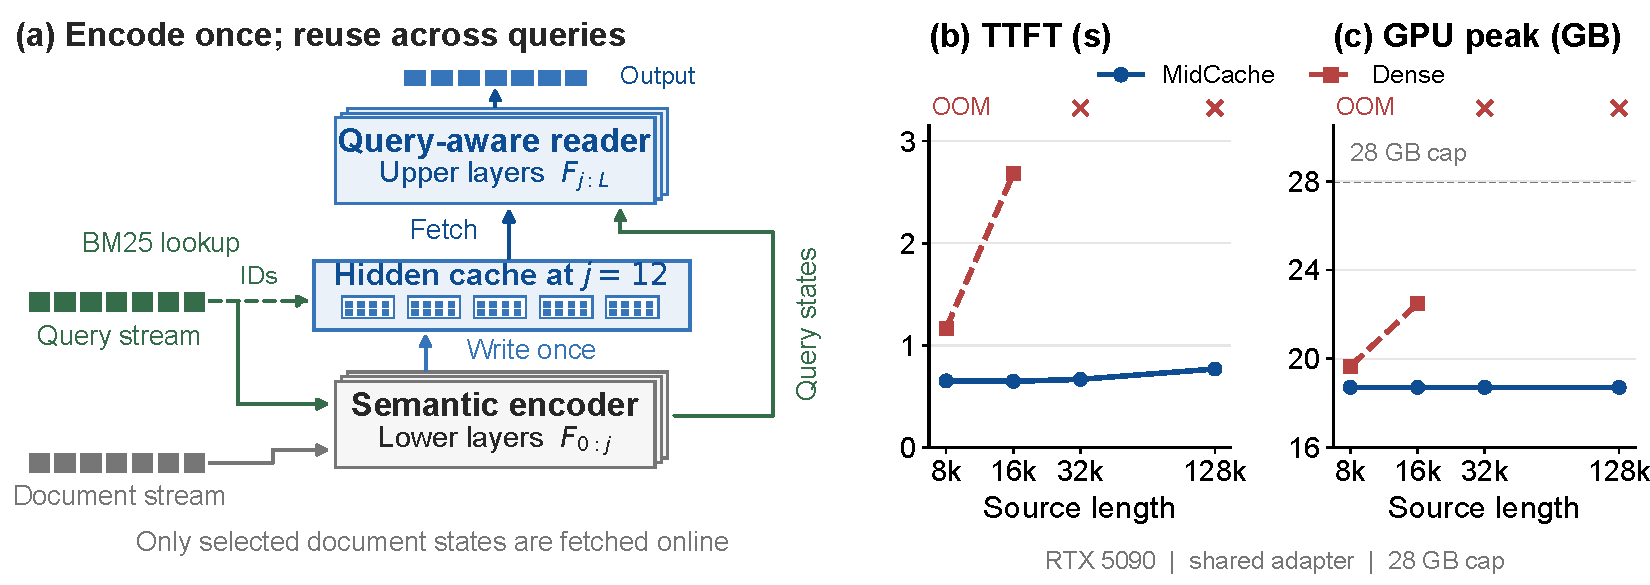
\includegraphics[width=\linewidth]{figures/teaser.pdf}
\caption{\textbf{A hidden cache between two parts of the LLM.} (a) The lower layers serve as a semantic encoder: their document states are cached once and reused by the upper reader. BM25 selects chunk IDs; only selected states are fetched. The query is also encoded before upper-layer continuation. (b--c) RTX 5090 measurements from Table~\ref{tab:infra}. TTFT includes retrieval, fetch, and query Write, but excludes document Write. GPU peaks include weights. Crosses mark actual Dense OOMs under the 28 GB allocator cap, without numerical values or extrapolation.}
\label{fig:teaser}
\end{figure}


We test both parts of this argument: whether intermediate states carry useful semantic information, and whether a decoder can reuse them efficiently. Layerwise probes motivate the encoder view; continuation checks, split-depth tests, and same-evidence comparisons evaluate the cache interface itself. MidCache reduces selected-pack prefill time on Qwen3-8B, with a measurable RULER accuracy cost. Independently encoded chunks also lose cross-chunk context, making quality task-dependent and motivating suffix adaptation and Write-context controls. The encoder view is a reusable computation boundary, not a claim that semantic processing ends at a universal layer.

Deployment depends on reuse. Residuals are smaller than full-depth KV but larger than token IDs, and construction must be amortized over future queries. Accounting for Write, fetch, Read, and decode shows how source length, output length, and storage placement affect this crossover. Tests with latency-calibrated chunk budgets then assess whether spending the saved computation on additional evidence improves quality.

\paragraph{Contributions.}
\begin{itemize}[leftmargin=1.3em,itemsep=2pt,topsep=3pt]
\item \textbf{A semantic-encoder cache.} MidCache turns lower-layer document representations into persistent memory and reuses them through the decoder's own upper layers.
\item \textbf{An adapted reader and a testable interface.} Suffix self-distillation, continuation checks, and fixed-evidence context/depth controls establish how independently encoded states can be read and where fidelity is lost.
\item \textbf{Measured conditions for useful reuse.} Repeated-query accounting and latency-calibrated budget comparisons quantify both amortization and the cases where raw replay remains preferable.
\end{itemize}
\FloatBarrier

\section{Related Work}
\label{sec:related}
\paragraph{Semantic representations and activation reuse.}
Layer interventions suggest a progression from contextual feature construction toward vocabulary-aligned prediction \citep{stagesofinference}, motivating reuse before the final readout. ReadOnce encodes documents into compressed, task-independent representations consumed by representation-plus-text models \citep{readonce}. Embedding Recycling caches intermediate activations and trains task-specific adapters above the frozen prefix \citep{embeddingrecycling}. LLMCache matches input fingerprints to reusable activation banks at different layers \citep{llmcache}. These works establish that intermediate computation can be reused. MidCache develops this idea as a document interface within an autoregressive decoder: one persistent residual per token is retrieved across queries and read by the model's own upper blocks.

\paragraph{Hidden states for KV restoration.}
HCache stores intermediate activations across layers and reconstructs layerwise KV through coordinated transfer and computation \citep{hcache}. KV-Direct reconstructs KV on demand from residual checkpoints \citep{kvdirect}. Their objective is to restore attention state for subsequent inference. MidCache instead stores one layer's document residuals and directly executes the remaining blocks after retrieval. This changes both the persistent object and the computation left online; independent Write also introduces a fidelity cost that restoration from compatible checkpoints need not incur.

\paragraph{Reusing document KV.}
Prompt Cache defines reusable prompt modules with explicit positional accounting \citep{promptcache}. Block-Attention trains blockwise attention for independently reusable passage KV \citep{blockattention}. TurboRAG assembles precomputed chunk KV using independent attention and reordered RoPE \citep{turborag}. CacheBlend selectively recomputes tokens to restore cross-chunk dependencies \citep{cacheblend}. EPIC combines sparse attention recomputation with semantic chunking for position-independent reuse \citep{epic}. APE aligns independently encoded contexts through a shared prefix and attention calibration \citep{ape}. MEPIC combines page-aligned storage, blockwise recomputation, and RoPE fusion to share cached chunks \citep{mepic}. RAGCache organizes retrieved knowledge states in a tree across GPU and host memory \citep{ragcache}. Cache-Craft estimates chunk-cache reusability and coordinates selective repair, placement, and eviction \citep{cachecraft}. These systems motivate accounting for transfer and repair alongside saved encoding. MidCache trades their full-depth KV object for a smaller residual cache and more upper-layer computation per query.

\paragraph{Learned memory and readers.}
KV Packet uses learned soft-token adapters around immutable document KV to bridge independently encoded contexts \citep{kvpacket}. Cartridges optimizes a compact corpus-specific KV cache through synthetic conversations and context distillation \citep{cartridges}. SemPIC distills a LoRA writer that produces reusable per-layer KV for an unchanged reader \citep{sempic}. MemoryLLM learns a fixed-size latent memory pool that updates with incoming text \citep{memoryllm}. LongMem couples a frozen memory encoder with an adaptive residual side-network for retrieval and reading \citep{longmem}. XC-Cache adds cross-attention modules to read cached context encodings \citep{xccache}. MidCache adapts the existing decoder suffix to consume the lower prefix's residuals, retaining one vector per document token without a separate reader network or corpus-specific cache optimization.

\paragraph{Selecting evidence and retaining KV.}
RAG retrieves text that the generator encodes for each request \citep{rag}. ILRe retrieves salient tokens using a chosen intermediate layer's key cache \citep{ilre}. REFORM gathers relevant tokens from incrementally compressed context and selectively recomputes their KV \citep{reform}. GemFilter uses early-layer attention to select tokens for a shorter generation context \citep{gemfilter}. InfLLM retrieves token-relevant distant memory blocks for attention within a limited context window \citep{infllm}. StreamingLLM retains initial attention sinks and a recent window \citep{streamingllm}. SnapKV selects per-head KV positions using attention from a prompt-end observation window \citep{snapkv}. PyramidKV assigns larger KV budgets to lower layers and smaller budgets to upper layers \citep{pyramidkv}. MiniCache merges similar KV states across neighboring layers \citep{minicache}. MidCache combines evidence selection with persistent encoder outputs: selection determines \emph{which} evidence is processed, while the split determines \emph{how much} encoding is repeated. Our same-evidence replay control separates these effects.

\section{Motivation}
\label{sec:motivation}
\paragraph{Semantic information is available before the final readout.}
The lower transformer blocks encode token identity and context into a residual representation that subsequent blocks refine for prediction, consistent with layerwise studies of feature construction and readout \citep{stagesofinference}. Our probes on SST2, WiC, and RTE examine information accessible from these states. SST2 probe accuracy peaks near 0.90, compared with approximately 0.71 for lexical features (Appendix~\ref{app:semantic-probes}). This motivates treating the lower prefix as a semantic encoder whose output can be cached before the final LM head. The claim concerns accessible representations, not a universal depth at which understanding is complete.

\paragraph{The remaining layers must be able to read the cached encoding.}
Storing semantic information and making it usable by a particular reader are different requirements. Independent chunk encoding enables query-independent reuse, but omits lower-layer attention to earlier document chunks. The upper reader must therefore consume states that differ from those in a continuous forward pass. This motivates adapting the suffix while preserving causal interaction across the selected chunks and query. We test readability directly with matched replay and context controls: LongEval's 64--76\% accuracy after a retrieval hit shows why a useful representation alone does not guarantee a correct answer.

\paragraph{Saved Read work must repay preparation.}
Placing a cache after the encoder removes its document computation from subsequent requests. A deeper split prepays more layers, while every query still runs the reader on the selected states. This requires upfront Write and storage, so reuse frequency, output length, and fetch cost determine the end-to-end benefit. We first hold evidence fixed to measure the saved encoding work and its quality cost, then test amortization and whether replay can answer more accurately with fewer chunks under latency-calibrated budgets.

\section{Methodology}
\label{sec:method}
MidCache implements the encoder--cache--reader view within one decoder: the lower prefix encodes document chunks for persistent reuse, and the upper suffix reads selected encodings with the current query. Both parts use the original transformer blocks.
\begin{figure}[t]
\centering
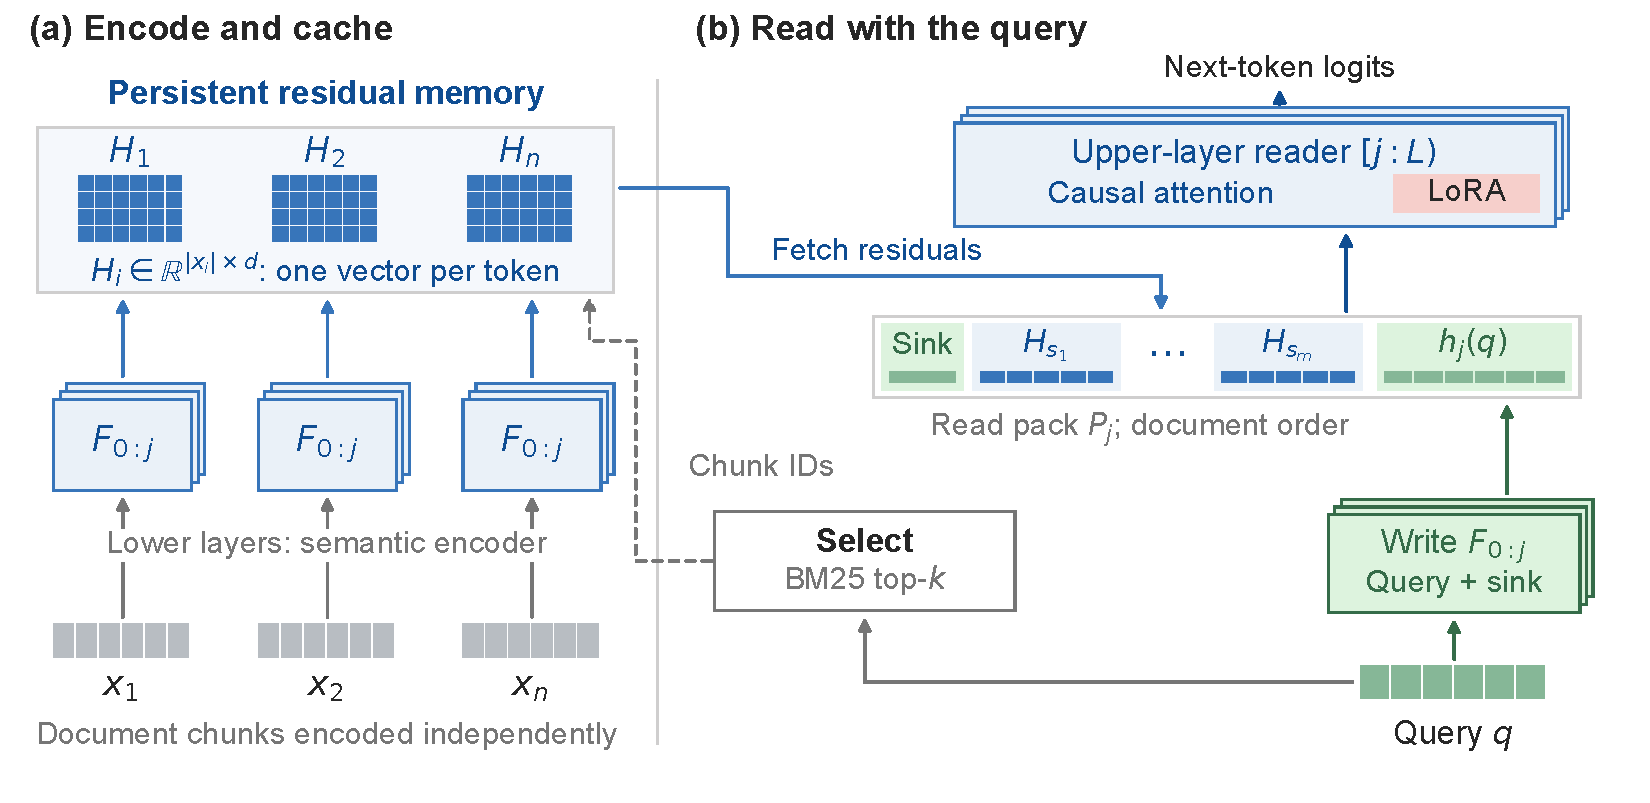
\includegraphics[width=\linewidth]{figures/architecture.pdf}
\caption{\textbf{CoMem reuses document computation at a residual interface.} (a) The shared lower-layer semantic encoder writes each chunk into a residual matrix $H_i$. (b) The query selects at most $k$ chunk IDs (dashed path). Cached encodings (blue) join separately encoded sink/query states (green), in document order, for causal processing by the upper reader $[j{:}L)$. Suffix LoRA adapts this reader to independently written states; the frozen variant omits it. Overlap-Write adds left context in (a) while retaining only target-token states.}
\label{fig:arch}
\end{figure}

Let a decoder have $L$ blocks, hidden width $d$, and half-open layer ranges. The residual $h_j$ is the input to block $j$, after blocks $[0{:}j)$ have run. A document of $N$ tokens is divided into chunks $x_i$ of at most $c$ tokens. The split $j$, chunk size $c$, and retrieval budget $k$ define the reusable interface.

\paragraph{Choosing the split.}
The principal Qwen3-8B configuration uses $j=12$, prepaying 12 of 36 blocks and leaving 24 for Read. Section~\ref{sec:depth-choice} explains this operating choice with a depth sweep; Appendix~\ref{app:split-choice} specifies the implementation's default rule.

\subsection{Write once, Read across queries}
\label{sec:interface}
\paragraph{Write: cache the semantic encoder's output.}
For $j>0$, each chunk is processed independently with rotary positions restarted at zero. We retain $H_i=F_{0:j}(x_i)\in\mathbb{R}^{|x_i|\times d}$, where $F_{0:j}$ denotes the embedding and lower-block computation. This is one vector \emph{per token}. A separate token-ID BM25 index maps the question to chunk IDs, which address the stored residuals. At $j=0$, the stored object is token IDs and document computation is deferred to each query.

\paragraph{Retrieval policy.}
The principal selector uses deterministic token-ID BM25 \citep{bm25}, top-12 chunks, hop width four, and three frontier-expansion rounds. The first round scores the question; subsequent rounds use newly selected chunks as the query frontier, deduplicate IDs, and break ties by document index. Retrieval uses CPU lookups without model forward passes; it addresses the cached states through chunk IDs rather than comparing residual vectors directly.

\paragraph{Select and Read: continue through the upper reader.}
Given a question, the selector returns at most $k$ chunk IDs, sorted back into document order. Let $q$ be the online query segment and $s$ the one-token sink. For $j>0$, both are encoded through the lower blocks independently of the stored chunks. The reader constructs
\begin{equation}
 P_j=[h_j(s);\,H_{s_1};\ldots;H_{s_m};\,h_j(q)],
 \qquad m\leq k,
 \label{eq:pack}
\end{equation}
and executes $F_{j:L}$ with fresh contiguous Read positions. Attention is causal: later chunks use earlier chunks, and query tokens use all selected chunks. Earlier document tokens do not attend to the later query. Each generated token still traverses all $L$ layers: lower-layer KV covers $q$ and the generated prefix, while upper-layer KV covers the selected pack and generated prefix. These KV caches are request-local; only document residuals persist across queries. Appendix~\ref{app:query-boundary} specifies benchmark query boundaries and sink conventions.

The matched $j=0$ reader assembles the same sink, chunk tokens, and query with the same order and causal mask, then executes the entire decoder. For the principal depth comparison, both endpoints carry the same suffix LoRA. Consequently, the comparison isolates the deployed depth interface without changing the selected evidence or adaptation parameters. It does not assume that independently written $h_j$ equals a continuous-prefix residual.

\paragraph{Relation to prefill and decode.}
Write--Read describes cross-query reuse. Online Read prefills the assembled states through the upper layers before autoregressive decode; it saves repeated document encoding, while generated tokens still use the complete decoder. Section~\ref{sec:infra} and Appendix~\ref{app:systems} distinguish this saved prefill work from TTFT and Write-inclusive E2E.

\paragraph{Storage and model-side work.}
For element size $b$, head width $d_{\mathrm{head}}$, $n_{\mathrm{kv}}$ KV heads, and $n_{\mathrm q}$ query heads, residual and full-KV bytes per token are $bd$ and $2bLn_{\mathrm{kv}}d_{\mathrm{head}}$. With $d=n_{\mathrm q}d_{\mathrm{head}}$,
\begin{equation}
 \frac{\mathrm{residual\ bytes/token}}{\mathrm{full\ KV\ bytes/token}}
 =\frac{d}{2Ln_{\mathrm{kv}}d_{\mathrm{head}}}
 =\frac{n_{\mathrm q}}{2Ln_{\mathrm{kv}}}.
 \label{eq:storage}
\end{equation}
For Qwen3-8B in bf16, this is 8 KiB versus 144 KiB per token. Residual bytes are independent of $j$ for the nonzero splits studied here; deeper caching changes prepaid computation, not tensor width. The $j=0$ token-ID endpoint is much smaller. The online pack length is bounded by $1+kc+|q|$, so model-side Read work is independent of $N$ for fixed $k,c,|q|$. Decode additionally depends on the generated prefix. Write, persistent storage, indexing, and selection still grow with the corpus.

\subsection{Adapt the suffix to independently written states}
\label{sec:distill}
The cached states encode document content, but independent Write changes the context seen below the split. We therefore train the reader to consume this interface using rank-32 LoRA on attention and MLP projections in blocks 12--35 of frozen Qwen3-8B \citep{lora,qwen3}. A $j=12$ student matches an adapter-disabled $j=0$ teacher on plain PG-19 windows \citep{pg19,distillation}. Each window supplies seven context chunks and a query chunk. The teacher processes the complete ordered pack causally through all layers. The student encodes each chunk, the sink, and the query independently below the split, then processes their assembled states causally in the adapted suffix. Both use the same token IDs and order; neither sees future tokens. Only query tokens contribute to the loss.

At token $t$, let $S_t$ contain the teacher's top-64 vocabulary indices. Teacher probabilities $p_t$ and student probabilities $q_t$ are separately renormalized on this same support. The token-mean objective is
\begin{equation}
 \mathcal{L}=\frac{1}{|Q|}\sum_{t\in Q}
 \left[0.6\,\mathrm{KL}(p_t\Vert q_t)+0.4\,\mathrm{KL}(q_t\Vert p_t)\right],
 \label{eq:distill}
\end{equation}
where $Q$ denotes query-token positions. This matches the conditional distributions on $S_t$, without constraining the student's total probability mass on that support. Post-training validation measures retained mass and full-vocabulary divergence (Appendix~\ref{app:distillation-validation}). Training uses 4,000 steps on 4,096-token windows, without retrieval, synthetic long-context data, or benchmark supervision. Appendix~\ref{app:protocol} specifies visibility, positions, and optimization. The adapter-disabled training teacher is distinct from the adapter-matched evaluation endpoint.

All full-suite results use independently written, nonoverlapping chunks. To diagnose sensitivity to encoding context, a separate Overlap-Write variant adds a short left prefix during Write and discards its states (Appendix~\ref{sec:overlap}); Section~\ref{sec:diagnosis} reports its quality and cost.

\section{Experiments}
\label{sec:experiments}
We evaluate answer quality, efficiency and amortization, split-depth choice, cache-boundary fidelity, and the use of saved time for additional evidence.
\paragraph{Setup.}
We use Qwen/Qwen3-8B, frozen except for the suffix LoRA, with $j=12$, $c=512$, iterative BM25 top-12, a one-token sink, greedy decoding, and plain-text prompts unless stated otherwise. Evaluation covers RULER, LongEval, six LongBench QA datasets, BABILong, and all 1,986 LoCoMo questions \citep{ruler,longchat,longbench,babilong,locomo}. Main-table RULER averages single-2, multikey-1, and variable tracking across five lengths from 8k to 128k, with 100 examples per cell. Appendix~\ref{app:protocol} specifies generation limits, sink conventions, metrics, and control cohorts.

\begin{table}[htbp]
\centering
\caption{\textbf{Cross-benchmark accuracy under the plain-text protocol.} Both CoMem variants use split depth $j=12$. All scores are on a 0--100 scale ($\uparrow$). Avg. is the descriptive, unweighted mean of the five benchmark scores. Best and second-best values in each column are \textbf{bold} and \underline{underlined}.}
\label{tab:accuracy}
\vspace{4pt}
\small
\setlength{\tabcolsep}{3pt}
\renewcommand{\arraystretch}{1.16}
\begin{tabularx}{\linewidth}{>{\hsize=2.05\hsize\linewidth=\hsize\raggedright\arraybackslash}X*{6}{>{\hsize=.825\hsize\linewidth=\hsize\raggedleft\arraybackslash}X}}
\toprule
\multirow{2}{*}{\textbf{Method}} & \multicolumn{5}{c}{\textbf{Benchmark scores}} & \multirow{2}{*}{\textbf{Avg.}}\\
\cmidrule(lr){2-6}
 & RULER & LongEval & LongBench & BABILong & LoCoMo & \\
\midrule
KV-Direct & \underline{78.80} & \underline{65.2} & \textbf{12.17} & \textbf{63.00} & \underline{34.59} & \underline{50.75}\\
InfLLM & 77.83 & 21.6 & 11.86 & \underline{59.52} & 22.21 & 38.60\\
StreamingLLM & 23.37 & 30.8 & 11.11 & 48.14 & 25.63 & 27.81\\
MemoryLLM$^{\dagger}$ & 16.55 & 13.6 & 9.01 & 30.00 & 16.11 & 17.05\\
HCache-style$^{\ddagger}$ & 3.73 & 0.0 & 9.20 & 33.71 & 8.11 & 10.95\\
\midrule
CoMem (without LoRA) & 16.87 & 0.2 & 9.86 & 37.48 & 24.52 & 17.78 \\
\rowcolor{resultshade}
\textbf{CoMem} & \textbf{97.05} & \textbf{69.0} & \underline{12.01} & 50.43 & \textbf{38.27} & \textbf{53.35}\\
\bottomrule
\end{tabularx}
\par\vspace{3pt}
\begin{minipage}{\linewidth}
\footnotesize
RULER: common 15-cell macro; LongEval: 8k--128k; LongBench: six-dataset macro F1; BABILong: three tasks over seven lengths; LoCoMo: Judge over 1,986 items. Replay controls are in Appendix~\ref{app:diagnostics}. KV-Direct is the full-context recomputation reference, unextended beyond 40,960 tokens; baseline implementations are specified in Appendix~\ref{app:protocol}.\\[1pt]
$^{\dagger}$Different backbone. $^{\ddagger}$Retrieval-free HCache-style checkpoint, distinct from the same-split adapter control and native HCache.

\end{minipage}
\end{table}

\subsection{Accuracy: reading the cached semantic encodings}
\label{sec:quality}
Table~\ref{tab:accuracy} compares seven configurations across five benchmarks. MidCache has the highest descriptive average, although full-context KV-Direct is stronger on BABILong and slightly stronger on LongBench. MidCache without LoRA scores 16.87 on RULER and 0.2 on LongEval, showing that the unadapted interface performs poorly on these tasks. This overview summarizes operating points; paired controls below isolate depth reuse.

The matched replay experiment uses separately sampled RULER examples with single-3 (Appendix~\ref{app:diagnostics}). Both arms share the checkpoint, adapter, examples, selected chunks, order, sink, and mask. Replay reaches 99.19 versus MidCache's 96.07: a 3.12-point fidelity cost at fixed evidence (95\% bootstrap interval $[2.36,3.93]$). This is a separate cohort from Table~\ref{tab:accuracy}.

The cost depends on the task. LongEval drops from 97.2 to 69.0 and LoCoMo Judge from 41.59 to 38.27. On the same 1,150 LongBench examples, unadapted replay and MidCache score 12.18 and 12.01 macro F1; both remain low. Strict PG-19 overlap filtering retains 1,053 examples and gives 12.21 and 12.05, preserving this near tie and MidCache's 2.15-point gain over its no-LoRA variant (Appendix~\ref{app:clean-longbench}). BABILong favors full-context KV-Direct on qa1/qa2 and MidCache on qa5. These natural-task replay references do not all share the RULER control's adapter setting, so they measure deployment configurations rather than one adaptation-matched effect.

Selection can nevertheless improve over processing the entire source. MidCache exceeds unextended KV-Direct on the main-table RULER aggregate and the no-chat LoCoMo Judge score. This is the combined effect of selection, adaptation, and the residual interface. It is not evidence that depth reuse itself improves accuracy: raw replay of selected evidence is stronger. The LoCoMo ordering is also prompt-dependent; with native chat formatting, KV-Direct scores 38.22 and MidCache 37.76 (Appendix~\ref{app:stats}).

Length extension changes the full-context reference. Qwen3-8B's native window is 40,960 tokens. In the separate factor-4 YaRN comparison, full-context KV-Direct reaches 100 on 128k single-needle retrieval, versus MidCache's 98, while MidCache is stronger on variable tracking (99.0 versus 57.8). SnapKV and PyramidKV also perform strongly after full-prompt prefill on the common shorter support. These results bound the claim to selected evidence and the measured systems trade-off, rather than universal accuracy gains beyond a position limit.

\subsection{Efficiency: reusing lower-layer document encoding}
\label{sec:infra}
\begin{table}[htbp]
\centering
\caption{\textbf{Infrastructure cost across three measurement settings.} Methods are compared within each panel; timing boundaries and hardware differ across panels. Lower latency and peak memory are better ($\downarrow$); higher speedup is better ($\uparrow$). Bold marks better results where both methods complete within each source length and panel.}
\label{tab:infra}
\vspace{4pt}
\small
\setlength{\tabcolsep}{5pt}
\renewcommand{\arraystretch}{1.15}
\begin{tabularx}{\linewidth}{ll*{5}{>{\raggedleft\arraybackslash}X}}
\toprule
\multicolumn{7}{l}{\textbf{(a) RTX 5090}\quad Full-source Dense; 28 GB memory cap}\\[2pt]
\multirow{2}{*}{\textbf{Source}} & \multirow{2}{*}{\textbf{Method}} & \multicolumn{3}{c}{\textbf{Latency (ms)} $\downarrow$} & \multicolumn{2}{c}{\textbf{Peak GPU (GB)} $\downarrow$}\\
\cmidrule(lr){3-5}\cmidrule(l){6-7}
 & & Prefill & TTFT & E2E$_{128}$ & Prefill & TTFT\\
\midrule
8k & Dense & 1194.4 & 1165.9 & 7987.6 & 19.66 & 19.66\\
\rowcolor{resultshade}
 & \textbf{MidCache} & \textbf{607.1} & \textbf{652.6} & \textbf{6331.6} & \textbf{18.68} & \textbf{18.71}\\
\midrule
16k & Dense & 2684.8 & 2681.3 & 12093.9 & 22.49 & 22.49\\
\rowcolor{resultshade}
 & \textbf{MidCache} & \textbf{606.5} & \textbf{648.0} & \textbf{6407.2} & \textbf{18.68} & \textbf{18.71}\\
\midrule
32k & Dense & OOM & OOM & OOM & OOM & OOM\\
\rowcolor{resultshade}
 & \textbf{MidCache} & 611.8 & 667.5 & 7026.1 & 18.68 & 18.71\\
\midrule
128k & Dense & OOM & OOM & OOM & OOM & OOM\\
\rowcolor{resultshade}
 & \textbf{MidCache} & 620.3 & 768.6 & 11426.8 & 18.68 & 18.71\\
\bottomrule
\end{tabularx}
\par\vspace{7pt}
\begin{minipage}[t]{0.485\linewidth}
\centering
\setlength{\tabcolsep}{2pt}
\begin{tabularx}{\linewidth}{l*{3}{>{\raggedleft\arraybackslash}X}}
\toprule
\multicolumn{4}{l}{\textbf{(b) B300}\quad 128k source}\\
\multicolumn{4}{l}{\textit{Store-ready prefill}}\\[2pt]
\textbf{Method} & \textbf{Latency} & \textbf{Peak GPU} & \textbf{Speedup}\\
 & (ms) $\downarrow$ & (GB) $\downarrow$ & $\uparrow$\\
\midrule
Dense & 15,919 & 62.03 & $1.00\times$\\
\rowcolor{resultshade}
\textbf{MidCache} & \textbf{194.8} & \textbf{18.71} & $\mathbf{81.7}\times$\\
\bottomrule
\end{tabularx}
\end{minipage}\hfill
\begin{minipage}[t]{0.485\linewidth}
\centering
\setlength{\tabcolsep}{2pt}
\begin{tabularx}{\linewidth}{l*{3}{>{\raggedleft\arraybackslash}X}}
\toprule
\multicolumn{4}{l}{\textbf{(c) B200}\quad 128k source}\\
\multicolumn{4}{l}{\textit{Write-inclusive pipeline}}\\[2pt]
\textbf{Method} & \textbf{Latency} & \textbf{Peak GPU} & \textbf{Speedup}\\
 & (ms) $\downarrow$ & (GB) $\downarrow$ & $\uparrow$\\
\midrule
Dense & 6,035 & 89.39 & $1.00\times$\\
\rowcolor{resultshade}
\textbf{MidCache} & \textbf{2,202} & \textbf{18.54} & $\mathbf{2.74}\times$\\
\bottomrule
\end{tabularx}
\end{minipage}
\par\vspace{4pt}
\begin{minipage}{\linewidth}
\footnotesize
\textbf{(a)} Dense processes the full source; MidCache resumes from cached $j=12$ residual states of 12 selected chunks. Both share the adapter. The 28 GB CUDA allocator cap includes weights, KV, and temporaries; OOM denotes an actual failure. Prefill starts GPU-ready; TTFT adds transfer and MidCache retrieval/query Write. E2E$_{128}$ includes document preparation and 128 output tokens. Model load, tokenization, and external I/O are excluded. Three processes and three documents; protocol and OOM attempts are in Appendix~\ref{app:local-infra}. GPU peaks are allocated bytes including weights (decimal GB); the adapter is shared with Table~\ref{tab:accuracy}; these cost inputs are unscored.\\[1pt]
\textbf{(b)} Same adapter; full prompt versus cached residual states at $j=12$. Document/query Write and fetch excluded; three processes, three documents, three repeats each. \textbf{(c)} Same adapter; document Write included, index construction and external I/O excluded. Full protocols: Appendix~\ref{app:systems}. Persistent storage is separate: residuals 8 KiB/token, token IDs 4--8 B/token, full KV 144 KiB/token.
\end{minipage}
\end{table}

Table~\ref{tab:infra}(a) compares full-source Dense with MidCache's 12-chunk residual Read on RTX 5090 under a 28 GB cap. The adapter matches Table~\ref{tab:accuracy}; the cost inputs are separate and unscored. Charging full document preparation and 128 output tokens, MidCache's E2E speedup is $1.26\times$ at 8k and $1.89\times$ at 16k. Dense exceeds the cap at 32k/128k, with no inferred latency or speedup. These complete configurations combine selection and depth reuse; Appendix~\ref{app:local-infra} also holds evidence fixed.

In the H20 same-pack, same-adapter depth comparison, selected-pack prefill falls from 931.9 to 664.4\,ms. The $1.403\times$ speedup accompanies the 3.12-point matched RULER loss above. This timer excludes selection, reusable Write, fetch, and decode. Adding the measured autoregressive decode components reduces the prefill-plus-decode speedup to approximately $1.07$--$1.09\times$.

The B300 same-adapter comparison gives 15,919 versus 194.8\,ms ($81.7\times$), combining selection and depth reuse while excluding preparation and fetch. The B200 same-adapter pipeline includes document/query Write, CPU retrieval, and upper-layer Read: speedup reaches $2.74\times$ at 128k, but MidCache is slower at 8k/16k. Index construction and external I/O remain excluded. Appendix~\ref{app:systems} specifies these distinct timing boundaries; the ratios do not describe one common workload.

\paragraph{Residuals versus chunk KV.}
The matched chunk-KV control tests all three paths with and without the principal adapter (Appendix~\ref{app:chunkkv}). MidCache's LongEval accuracy of 72.67 is close to unadapted chunk-KV's 73.00, at 8 versus 144 KiB per token. Applying the MidCache-trained adapter lowers chunk-KV to 55.67. On RTX 5090 at 32k with the shared adapter, chunk-KV has lower TTFT (400 versus 613\,ms), but MidCache has lower Write-inclusive E2E for 128 output tokens (7.01 versus 11.69\,s). This measures a synchronous reference, not native CacheBlend performance.

\paragraph{When does preprocessing amortize?}
Let $W_C$ be MidCache's one-time preparation cost, $I_0$ the raw-replay preparation cost, and $T_C,T_0$ the measured per-query costs, including fetch, Read, and decode. With common selection costs cancelling, the crossover is
\begin{equation}
 Q^\star=\frac{W_C-I_0}{T_0-T_C},\qquad T_0>T_C.
 \label{eq:breakeven}
\end{equation}
Round this threshold up for integer reuse counts. CPU-pinned storage breaks even at 8.9--10.9 queries at 32k for outputs up to 128 tokens, rising to 27.6--37.4 at 128k. Nonpositive per-query savings with costlier preparation yield no finite crossover, as in the 32k GPU-resident case with 512 output tokens. Appendix~\ref{app:systems} covers larger stores and other placements. These single-query measurements do not establish throughput or tail latency.

\subsection{Choosing the cache depth: why $j=12$?}
\label{sec:depth-choice}
We use the lower-third default, $j=\operatorname{round}(0.33L)=12$ for the 36-layer Qwen3-8B. Table~\ref{tab:depth-choice} shows the quality--Read trade-off. Moving from $j=6$ to $12$ saves 20\% of Read time at a 2.22-point RULER cost; $j=18$ is faster but loses much more quality. Thus $j=12$ prepays useful encoder work while retaining 24 reader blocks, and is fixed across the main benchmarks. Stricter quality budgets may favor shallower splits. Each split has its own adapter; this supports a practical operating choice, not a universal semantic boundary or a validated optimum.
\begin{table}[htbp]
\centering
\caption{\textbf{Depth sensitivity on Qwen3-8B.} Each split uses a separately distilled suffix adapter with different parameter counts. Read is selected-pack prefill, excluding selection, Write, fetch, and decode; speedup uses each split's own full-replay reference. Shading marks the main operating point. Full settings and uncertainty: Appendix~\ref{app:diagnostics}, Table~\ref{tab:multidepth}.}
\label{tab:depth-choice}
\small
\setlength{\tabcolsep}{4pt}
\renewcommand{\arraystretch}{1.08}
\begin{tabularx}{\linewidth}{l*{4}{>{\raggedleft\arraybackslash}X}}
\toprule
Split $j$ & RULER B $\uparrow$ & LoCoMo $\uparrow$ & Read (ms) $\downarrow$ & Speedup $\uparrow$ \\
\midrule
6 & 98.29 & 40.38 & 830.3 & $1.166\times$ \\
9 & 97.55 & 39.02 & 748.3 & $1.273\times$ \\
\rowcolor{resultshade}
\textbf{12} & 96.07 & 38.27 & 664.4 & $1.403\times$ \\
18 & 55.41 & 28.65 & 499.5 & $1.807\times$ \\
\bottomrule
\end{tabularx}
\end{table}


\subsection{Fidelity: context and adaptation at the cache boundary}
\label{sec:diagnosis}
The encoder view predicts reusable semantic content, but not equivalence to a continuous forward pass. We examine whether losses arise from continuation, encoding context, or the reader's ability to use independently written states.
\paragraph{Continuation correctness and missing context are separate.}
A continuous-prefix oracle computes the lower layers on the selected assembled sequence for every query and then resumes at $h_{12}$. It exactly recovers raw replay on the paired control examples. This verifies continuation with compatible states, but forfeits their cross-query reuse. A separate context--position control keeps selected chunks, the suffix adapter, and upper-layer causal connectivity fixed while varying lower-layer context scope and upper-layer RoPE coordinates.

On the paired 8k/16k multikey cohort, chunk-local Write reaches 92.5 with local Read positions and 88.0 with document-origin positions. Full-document lower-layer context reaches 100.0 under both conventions. However, this control also contextualizes the query and retains full-document lower-layer KV during decode. It establishes recovery under broader context, not an isolated effect of cached document states or a fixed-evidence comparison. Changing positions alone does not repair the loss (Appendix~\ref{app:diagnostics}).

\paragraph{A local context extension is task-dependent.}
Overlap-Write with 32 left-context tokens raises multikey accuracy from 92.5 to 98.5 (paired 95\% gain interval $[3.0,9.5]$). Only document-block encoding changes; query Write, lower-layer decode, stored bytes, and the online computation graph remain fixed. The theoretical lower-layer Write FLOP ratio is $1.057\times$, with larger wall-clock overhead. However, a fixed-$w=32$ confirmation on 300 fresh LongEval examples reduces accuracy from 72.67 to 62.33 ($-10.33$ points, $[-16.33,-4.33]$). On all 200 Qasper examples, F1 changes from 11.37 to 10.76 ($-0.61$, $[-1.43,0.21]$). On a prespecified 20-example RTX 5090 subset, overlap adds 17.9--19.4\% to document Write and 1.1--4.2\% to E2E, with unchanged stored bytes (Appendix~\ref{app:overlap-cost}). The repair is task-dependent.

\paragraph{Adaptation and interaction matter independently.}
At fixed $j=12$, suffix distillation raises LoCoMo Judge from 24.52 to 38.27 and lowers held-out PG-19 full-vocabulary teacher--student KL from .442 to .304 (Appendix~\ref{app:distillation-validation}). Full causal cross-chunk processing separately improves multikey accuracy over block-diagonal processing with the same query access (Appendix~\ref{app:diagnostics}).

\subsection{Can saved encoding time buy useful evidence?}
\label{sec:equallatency}
On three disjoint 32k multikey documents, H20 first-logit latency including selection/fetch is 703.7\,ms for replay with ten chunks and 699.8\,ms for CPU-pinned MidCache with twelve. We fix these latency-calibrated budgets before comparing quality on nine equally weighted task--length cells. Their per-cell latencies are unreported. With iterative BM25 for both arms, replay scores 64.78 versus MidCache's 53.22: a $-11.56$-point difference (hierarchical 95\% interval $[-18.67,-5.11]$), remaining negative after dropping any single cell. Full-depth replay is preferable on this mixture.

Replacing only replay's selector with frozen BGE changes its score to 54.22. The resulting one-point edge has a hierarchical interval spanning zero. This is a comparison of selector choices, not a same-evidence test of depth. The LoCoMo slice contains one conversation, further limiting generalization. Thus saving encoder work can increase the evidence budget, but additional chunks do not necessarily offset the residual interface's fidelity cost. Appendix~\ref{app:equal} gives absolute latencies, cell deltas, and the resampling protocol.

\section{Conclusion}
\label{sec:conclusion}
MidCache turns the semantic-encoder role of early transformer layers into reusable document memory. Intermediate residuals retain the output of document encoding; caching them lets later queries resume through the model's own upper layers with selected evidence. Suffix self-distillation makes independently encoded states more readable, while fixed-evidence controls quantify the resulting fidelity cost. The experiments demonstrate saved document computation and a smaller persistent object than full-depth KV, with end-to-end gains governed by reuse and preparation. This encoder--cache--reader view makes intermediate representations an explicit acceleration interface whose split depth and quality must be validated for the task.

\subsection*{Ethics statement}
CoMem inherits the underlying model's hallucination, bias, and unsafe-generation risks. Persistent residuals may disclose source information and should receive protections appropriate to the underlying text, including access control, tenant isolation, and deletion that accounts for cached dependencies. The study does not test inversion or membership-inference attacks. Experiments use released models, corpora, and benchmarks and collect no new human-subject data. Model weights, benchmark text, credentials, and private API responses remain subject to the source providers' access and redistribution terms.

\subsection*{Reproducibility statement}
Appendix~\ref{app:protocol} specifies inference and training settings; Appendices~\ref{app:diagnostics}--\ref{app:stats} provide detailed results, timing boundaries, and statistical procedures. The distillation validation, matched KV quality and cost controls, and three-method LongBench clean-subset analysis include saved per-example or per-token measurements. Protocols distinguish paired controls from descriptive comparisons and state their remaining coverage limits.

\bibliography{refs}
\bibliographystyle{unsrtnat}
\clearpage
\appendix
\FloatBarrier
\section{Experimental Protocol}
\label{app:protocol}
\subsection{Inference configuration}
The principal checkpoint is the released \texttt{Qwen/Qwen3-8B}, revision \texttt{b968826d9c46}. It has 36 layers, width 4096, 32 query heads, eight KV heads, and head width 128. Inference uses bf16 and SDPA. The native maximum position is 40,960, with RoPE base $10^6$ and no active scaling unless a YaRN arm is explicitly named. The study does not continue-pretrain the backbone.

\paragraph{Split-depth configuration.}
\label{app:split-choice}
The released model registry sets \texttt{DEFAULT\_RATIO=0.33} and maps Qwen3-8B explicitly to $j=12$; for an unlisted backbone, \texttt{--j auto} falls back to $\operatorname{round}(0.33L)$. Training and timing entry points also default to 12, while an explicit $j$ overrides the default. This is a deployment heuristic motivated by the depth--fidelity trade-off; the study does not establish it through probe-based or held-out benchmark selection. The main Qwen3-8B evaluations retain $j=12$ across tasks and source lengths, including the no-LoRA control; Table~\ref{tab:multidepth} reports sensitivity to alternative splits. Its separately trained adapters and varying parameter counts prevent interpreting the sweep as an equal-training-compute optimization or establishing a universally optimal depth.

The default writer independently encodes disjoint 512-token chunks through blocks 0--11, restarting positions at zero. It stores all target-token residuals in bf16. The reader orders selected chunks by document position, prepends the BOS sink, and appends the independently encoded query. The nominal cap is $1+12\times512+512=6{,}657$ tokens; shorter tails and queries produce observed means around 6.2--6.5k. Its causal mask allows later chunks to attend to earlier chunks. In the block-diagonal control, each chunk sees itself and the sink, while the final query still sees every chunk.

BM25 operates on token-ID documents and question token IDs, using $k_1=1.5$, $b=0.75$, and Robertson IDF with $+1$ smoothing. There is no lowercasing, stemming, or stop-word removal. The saved \texttt{rounds=0} setting means automatic $\lceil k/h\rceil$ rounds, not a single pass. With $k=12$ and hop width $h=4$, all five benchmark families use three rounds, with newly selected chunks forming the next frontier. Decoding is greedy without a chat template or thinking mode. The MidCache and MidCache without LoRA configurations both use $j=12$; Appendix~\ref{app:frozen-recheck} specifies the no-adapter evaluation protocol.

\paragraph{Persistence and query boundaries.}
\label{app:query-boundary}
The reusable interface accepts source and query separately: source tokenization and chunk boundaries are fixed before questions arrive. A chunk ID addresses both its token-ID retrieval metadata and its bf16 residual matrix. Changing only the upper-layer adapter or the selected IDs preserves the stored lower-layer states. Changing source tokens, chunk boundaries, split depth, lower-layer weights, or Write positions requires rebuilding the affected states; overlap also makes a chunk depend on its left prefix. The storage formula counts residual payload only, excluding token IDs, retrieval-index metadata, and request-local KV.

The released monolithic benchmark driver instead tokenizes the complete formatted prompt and takes its last chunk as $q$, with preceding chunks as candidate evidence. BM25 receives the bare question. Thus $q$ need not coincide with the question text: it can contain a document tail, and a question can straddle a chunk boundary. Any block containing query-dependent text must be rebuilt for that query. These formatted-example quality tests do not themselves measure cross-query reuse. The source/query-separated serving experiments measure reuse with fixed document blocks. All methods within each paired control share the same boundary.

The benchmark sink uses the tokenizer's BOS when available and otherwise the first formatted-input token. The Qwen3 tokenizer has no BOS ID. The overlap/KV confirmation and distillation validation instead explicitly use model BOS 151643, identically across their arms; their Qasper values therefore need not equal the main-table Qasper scores. This convention changes an input token, not the chunk selector or the number of sink positions.

\subsection{Suffix-adapter training}
The rank-32 LoRA has $\alpha=32$, zero dropout, and 58.20M trainable parameters (0.71\% of the model). It updates Q/K/V/O and gate/up/down projections only in layers 12--35. The adapter-disabled backbone is the frozen teacher. At every query token, teacher top-64 indices define the shared support used by Equation~\ref{eq:distill}; temperature is one and loss is averaged over query tokens. There is no auxiliary cross-entropy. Appendix~\ref{app:distillation-validation} measures support mass and full-vocabulary divergence on held-out books after training.

Training uses a 64-book PG-19 training subset in 4,096-token windows, partitioned into seven context chunks and one query chunk of 512 tokens each. Teacher and student share the sink, token IDs, chunk order, and query segment. The teacher disables the adapters and processes $[s;x_1;\ldots;x_7;q]$ from layer zero as one causal sequence. Its document positions see the sink and preceding document positions, but no query tokens; its query positions see all preceding document positions and their own causal prefix.

The student's lower layers instead process the sink, each context chunk, and the query as separate causal segments, without gradients or an added per-chunk sink. If $g(t)$ identifies a segment in the assembled order, lower-layer visibility is $u\le t$ and $g(u)=g(t)$; teacher and upper-layer visibility is simply $u\le t$. Write positions restart at zero for each segment. Upper-layer positions are contiguous across the 4,097-position pack, including the sink. Only the suffix adapter receives gradients. This is a causal teacher with broader document context than the student's lower layers, not a teacher with access to future query tokens.

During generation, the lower-layer KV cache contains the query and generated prefix; the upper-layer cache contains the sink, selected document states, query, and generated prefix. A new token uses its next query-local position below the split and its next pack position above it. The continuous-prefix evaluation oracle uses the same full-pack visibility as the teacher but retains the evaluation adapter, whereas training disables it.

AdamW uses $\beta=(0.9,0.95)$, zero weight decay, peak learning rate $10^{-4}$, 50 warmup steps, cosine decay to zero, clipping at 1.0, and seed 42. The backbone is bf16; adapter master parameters are fp32 and matrix products use bf16 autocast. The executed run uses non-reentrant gradient checkpointing, 4,000 steps, one GPU, one 4,096-token window per step, and no accumulation: 16.384M training tokens. The 7.232M-token corpus is traversed cyclically, without inserted document separators; the initial eight windows are skipped once and can recur after wrapping. Training peak allocated memory is 18.01 GiB. These settings follow the checkpoint configuration and executed training record; total compute across preliminary experiments is not reported.

\subsection{Benchmarks and scoring}
\begin{table}[htbp]
\centering
\small
\setlength{\tabcolsep}{4pt}
\begin{tabular}{@{}lll@{}}
\toprule
Benchmark & Support / aggregation & Generation \\
\midrule
RULER & 15 cells, 100/cell; cell macro & 48; VT 60 \\
LongEval & 100/length; five-length macro & 16; without LoRA 48 \\
LongBench & 1,150 examples; six-dataset F1 macro & 32/64/128 \\
BABILong & 21 cells, 100/cell; cell macro & 20 \\
LoCoMo & 1,986 items; item-weighted Judge & 48; scale study 512 \\
\bottomrule
\end{tabular}
\caption{Evaluation supports and maximum generated tokens. RULER uses official case-insensitive string matching; BABILong uses official answer comparison with task labels. LongEval extracts the first numeric answer, LongBench uses official multi-reference token F1, and LoCoMo combines semantic judging with local abstention scoring. RULER, LongBench, and BABILong use seed 42; LongEval uses seed 1234. Adapted runs use eight shards for RULER/LongEval and four for BABILong/LoCoMo. The three paired LongBench configurations and no-adapter runs use four shards throughout.}
\label{tab:eval}
\end{table}

RULER Cohort A uses \texttt{niah\_single\_2}, \texttt{niah\_multikey\_1}, and \texttt{variable\_tracking}. Cohort B uses an independently sampled \texttt{niah\_single\_3} cohort for the matched YaRN and raw-replay comparisons. Both average 15 cells across 8k, 16k, 32k, 64k, and 128k with 100 examples per cell. The MidCache means are 97.05 and 96.07, respectively. A and B are labels for these experimental sample sets, not official RULER variants or train/test splits. The main table uses the task--length support of set A, with independently sampled synthetic runs for the adapter and no-adapter configurations. Set B is reserved for paired replay and YaRN controls. These macros cover 8k--128k; no direct difference is taken between the two cohorts.

\paragraph{Baseline mechanisms and implementation scope.}
The released driver implements the KV-Direct quality reference as full-depth, full-context recomputation without retrieval or LoRA. It evaluates that recomputation endpoint rather than the native system's residual-checkpoint storage and restoration scheduler. The HCache-style overview evaluates a retrieval-free split checkpoint; it is distinct from the same-$j=12$ adapter diagnostic and does not reproduce native HCache. StreamingLLM's sink/window reference retains initial and recent token IDs before dense generation. The SnapKV/PyramidKV controls first prefill the complete prompt and then compress retained KV. MemoryLLM uses its separately released backbone, as marked in Table~\ref{tab:accuracy}. These implementation scopes prevent attributing native serving-system costs to the quality overview. Appendix~\ref{app:chunkkv} separately describes the same-evidence CacheBlend-style reference and its simplified repair policy.

LongEval's common-support mean covers 8k--128k. LongBench averages the six dataset F1 scores equally; the three-task LLoCO mean is kept separate. BABILong averages seven lengths per task and three tasks for the overview. LoCoMo's full-set Judge folds 1,540 answerable questions and 446 locally scored abstention questions into one item-weighted score.

\paragraph{Software and artifacts.}
The benchmark environments use Python 3.10+, PyTorch 2.10, Transformers 5.5.4, PEFT 0.10+, Datasets 2.14+, bf16, and SDPA unless specified otherwise. The three paired LongBench configurations, KV control, and no-adapter benchmark runs use the B300 environment in Appendix~\ref{app:frozen-recheck}; Appendix~\ref{app:systems} gives the device-specific timing environments. Reproduction requires the evaluation code, adapter configuration, saved predictions or permissible score records, judge decisions, and timing records. External data remain subject to their original providers' terms.

\FloatBarrier
\section{Depth and Write-Interface Diagnostics}
\label{app:diagnostics}
These controls test when an intermediate semantic encoding remains usable by the upper reader: continuation checks separate implementation correctness from missing context, and depth, adaptation, and attention ablations examine fidelity at the cache boundary.
\subsection{Matched replay and continuation}
\begin{table}[htbp]
\centering
\small
\setlength{\tabcolsep}{4pt}
\begin{tabular}{@{}lrrrrr@{}}
\toprule
Path & RULER B & MK 8/16k & Read ms & p10 & p90 \\
\midrule
Raw replay $j=0$ & 99.19 & 100.0 & 931.9 & 931.6 & 942.0 \\
Chunk-local $j=12$ & 96.07 & 92.5 & 664.4 & 663.8 & 667.1 \\
Continuous-prefix oracle & 99.19 & 100.0 & --- & --- & --- \\
\bottomrule
\end{tabular}
\caption{Matched replay and Write-side attribution. The oracle freshly computes the selected sequence's lower-layer states per query and is not a reusable Write. Quality uses the paired 1,500-example Cohort B; MK denotes the 200-example multikey subset. Read uses a separate fixed pack from 16k sources with the same adapter and excludes retrieval, reusable Write, and I/O.}
\label{tab:matched-detail}
\end{table}

The matched RULER-B control holds checkpoint, all 168 suffix-LoRA modules, example IDs, decode parameters, and selected chunk IDs, order, and tokens fixed. Across 1,500 paired examples, full replay reaches 99.19 and layer-12 replay 96.07. The reported paired-bootstrap gap is 3.12 points with 95\% interval $[2.36,3.93]$; the binary correctness comparison contains 83 full-only and one layer-12-only correct cases (exact McNemar $p=8.79\times10^{-24}$). The binary test and the fractional task-macro difference summarize different aspects of the outputs.

Latency is measured on an approximately 6.5k-token pack from 16k sources, in three independent processes with three warmups and 20 reads per process. Process-level speedup ratios range from 1.402 to 1.404. Total decode medians are about 2.76--2.86 seconds; including them reduces the ratio to about 1.07--1.09. A component measurement attributes most Read savings to the transformer suffix ($1.398\times$), with unchanged LM-head time. Retrieval, index construction, reusable store/query Write, and persistent I/O are outside the Read timer.

The continuous-prefix oracle runs the lower layers on the selected packed sequence for each query before resuming the suffix. It is bit-identical to full replay on the reported examples. This is a correctness check and an attribution reference; its fresh per-query prefix computation prevents the claimed cross-query lower-layer reuse. The deployable chunk-local path loses 7.50 points on pooled 8k/16k multikey examples ($n=200$, 95\% interval $[4.0,11.5]$).

\subsection{Context, positions, and local repair}
\label{sec:overlap}
\begin{table}[htbp]
\centering
\small
\setlength{\tabcolsep}{4pt}
\begin{tabular}{@{}lrr@{}}
\toprule
Lower-layer context & Local Read positions & Document-origin positions \\
\midrule
Chunk local & 92.5 & 88.0 \\
Full document + query & 100.0 & 100.0 \\
\bottomrule
\end{tabular}
\caption{Lower-layer context $\times$ upper-layer RoPE positions on paired 8k/16k multikey examples ($n=200$). Selected chunks, adapter, and upper-layer causal connectivity are fixed. The full-document arm also contextualizes the query and retains full-prompt lower-layer KV during decode; it is not a document-state-only intervention.}
\label{tab:context}
\end{table}

\begin{table}[htbp]
\centering
\small
\setlength{\tabcolsep}{4pt}
\begin{tabular}{@{}llrl@{}}
\toprule
Writer & Left context & Macro & Write FLOPs \\
\midrule
Chunk local & $w=0$ & 92.5 & $1.000\times$ \\
Overlap & $w=32$ & 98.5 & $1.057\times$ \\
Overlap & $w=64$ & 98.5 & $1.115\times$ \\
Overlap & $w=128$ & 99.0 & $1.229\times$ \\
Trained lower-layer writer & none & 98.5 & $1.000\times$ \\
Full-document control & full prefix & 100.0 & full-prefix forward \\
\bottomrule
\end{tabular}
\caption{Writer repair on the same paired synthetic multikey cohort. Overlap keeps persistent bytes, query Write, and the online computation graph fixed. FLOPs are theoretical lower-layer Write ratios; wall-clock overhead is larger. The final row also broadens query/decode context. The learned writer uses a separate lower-layer LoRA.}
\label{tab:overlap}
\end{table}

Overlap-Write is a diagnostic of lower-layer encoding context. For a chunk $x_i$ and up to $w$ preceding source tokens $\ell_i^{(w)}$, it stores
\begin{equation}
 H_i^{(w)}=\left.F_{0:j}([\ell_i^{(w)};x_i])\right|_{x_i},
 \label{eq:overlap}
\end{equation}
retaining only states belonging to $x_i$. Thus the persistent tensor and online pack have the same shapes as at $w=0$, but Write performs extra work. An edit to the left prefix also invalidates the dependent chunk. All full-suite results use $w=0$.

The context--position factorial holds selected chunk IDs, LoRA, and upper-layer causal connectivity fixed. Its full-document arm runs layers 0--11 causally over the complete formatted source and query in original positions, including unselected source tokens. It slices the sink, selected document spans, and query states from that forward into the upper-layer pack. The query is therefore document-contextual, not independently written. During generation, the lower layers retain the complete prompt KV and attend to it at document coordinates; the upper layers retain only the selected pack and generated prefix. This differs from the selected-pack continuous-prefix oracle above, and its lower-layer KV and per-token attention work grow with source length.

The position factor changes upper-layer RoPE coordinates from contiguous pack positions to original document positions, including during decode. The causal mask is constructed from contiguous pack indices in both cases, so gapped RoPE coordinates do not change attention connectivity. Full-document context adds 7.5 points under local positions and 12.0 under document-origin positions; changing positions alone lowers chunk-local accuracy by 4.5 points. The $+4.5$ interaction rejects a purely additive account on these 200 examples. Because the context factor also changes query states and lower-layer decode visibility, these results do not isolate document-cache fidelity or hold all visible evidence fixed.

Overlap instead changes only document-block Write. It prepends up to $w$ tokens immediately preceding the chunk in the original source, encodes the extended span causally with positions starting at zero, and discards prefix states. Prefix tokens may come from unselected chunks. Sink/query Write, lower-layer query-local decode, selected IDs, and stored tensor shapes remain fixed; encoded context does not. The $w=32$ gain is 6.0 points, with 95\% interval $[3.0,9.5]$. The FLOP ratios in Table~\ref{tab:overlap} are theoretical lower-layer Write ratios; chunk-level execution incurs larger wall-clock overhead. The separate lower-layer LoRA writer at step 2000 improves over chunk-local Write (McNemar $p=5\times10^{-4}$), with $p=0.25$ against the full-document control. This does not establish equivalence or natural-task generalization.

\paragraph{Independent LongEval and natural-QA confirmation.}
\label{app:overlap-confirmation}
\begin{table}[htbp]
\centering
\small
\setlength{\tabcolsep}{5pt}
\begin{tabular}{@{}lrrrr@{}}
\toprule
& \multicolumn{3}{c}{LongEval accuracy} & Qasper F1 \\
\cmidrule(lr){2-4}
Method & 8k & 16k & 32k & All 200 \\
\midrule
Replay ($j=0$) & 80.00 & 77.00 & 76.00 & 4.65 \\
MidCache ($w=0$) & 71.00 & 74.00 & 73.00 & 11.37 \\
MidCache ($w=32$) & 59.00 & 68.00 & 60.00 & 10.76 \\
\midrule
$\Delta(w32-w0)$ & $-12.00$ & $-6.00$ & $-13.00$ & $-0.61$ \\
95\% paired CI & $[-22,-2]$ & $[-15,3]$ & $[-25,-1]$ & $[-1.43,0.21]$ \\
\bottomrule
\end{tabular}
\caption{Independent fixed-$w=32$ confirmation using the principal suffix adapter in all three arms. LongEval has 100 fresh examples per length; Qasper uses all 200 LongBench examples. Selection, sink, and query tokens are paired. All scores are percentages. Intervals use 20,000 paired example bootstraps, without multiplicity correction. The overlap provides no positive generalization evidence on these tasks.}
\label{tab:overlap-confirmation}
\end{table}

We fix $w=32$ before evaluating 300 fresh LongEval examples (100 each at 8k/16k/32k, seed 20260913 with length offsets) and all 200 Qasper examples from LongBench. Replay, $w=0$, and $w=32$ share the principal suffix adapter, input IDs, iterative BM25 top-12 selection, source order, and query segment. Chunks have 512 tokens; the final formatted-input chunk is the query. The sink is explicitly model BOS 151643 in every arm. The multikey diagnostic uses the first input token as its sink when the tokenizer has no BOS ID. This sink difference and the independently sampled inputs prevent item-paired differences across tasks. Generation is greedy, plain-text, and capped at 16 tokens for LongEval and 128 for Qasper. All outputs reached these caps. Qasper uses the best token F1 over reference answers, not a judge.

Table~\ref{tab:overlap-confirmation} does not reproduce the multikey repair. LongEval macro accuracy falls from 72.67 to 62.33, a paired $-10.33$ points (95\% CI $[-16.33,-4.33]$, resampling within length); replay scores 77.67. There are 28 overlap-only correct and 59 baseline-only correct examples. Qasper changes from 11.37 to 10.76 F1, with a paired difference of $-0.61$ ($[-1.43,0.21]$); these low, capped-output scores do not support preserved general QA capability. Four Slurm B300 workers evaluate disjoint samples, saving 1,500 outputs. An independent CPU pass checks sample support, generated-ID decoding, selected IDs, and every score. Before evaluation, each worker verifies adapter-off replay against stock logits and cached generation against recomputation.

An exploratory boundary analysis finds improvement when the target record begins within a chunk's first 32 positions (20 examples: 45 to 80 accuracy), but degradation on the 290 records that do not cross a chunk boundary (74.48 to 63.10). These overlapping, small subgroups do not establish a mechanism. The overall negative result rules out treating short overlap as a general repair under this protocol.

\paragraph{Quality and Write-inclusive cost on the same examples.}
\label{app:overlap-cost}
\begin{table}[htbp]
\centering
\small
\setlength{\tabcolsep}{4pt}
\begin{tabular}{@{}lrrrrrr@{}}
\toprule
Method & Quality & Write (ms) & TTFT (ms) & Online (s) & E2E (s) & GPU (GB) \\
\midrule
\multicolumn{7}{@{}l}{\textit{LongEval 8k ($n=5$)}} \\
Replay & 80.00 & 0.0 & 860.0 & 6.854 & 6.855 & 18.89 \\
MidCache & 100.00 & 351.1 & 647.7 & 6.032 & 6.383 & 18.59 \\
MidCache ($w=32$) & 80.00 & 419.2 & 647.1 & 6.035 & 6.456 & 18.59 \\
\addlinespace[3pt]
\multicolumn{7}{@{}l}{\textit{LongEval 16k ($n=5$)}} \\
Replay & 80.00 & 0.0 & 868.9 & 6.861 & 6.862 & 18.90 \\
MidCache & 60.00 & 706.1 & 655.3 & 6.056 & 6.767 & 18.59 \\
MidCache ($w=32$) & 40.00 & 843.3 & 653.2 & 6.070 & 6.916 & 18.59 \\
\addlinespace[3pt]
\multicolumn{7}{@{}l}{\textit{LongEval 32k ($n=5$)}} \\
Replay & 100.00 & 0.0 & 876.9 & 6.899 & 6.900 & 18.92 \\
MidCache & 20.00 & 1416.6 & 661.2 & 6.071 & 7.475 & 18.62 \\
MidCache ($w=32$) & 80.00 & 1687.9 & 662.7 & 6.071 & 7.788 & 18.62 \\
\addlinespace[3pt]
\multicolumn{7}{@{}l}{\textit{Qasper ($n=5$)}} \\
Replay & 16.36 & 0.0 & 537.4 & 5.556 & 5.556 & 18.26 \\
MidCache & 21.48 & 154.2 & 422.6 & 5.344 & 5.497 & 18.06 \\
MidCache ($w=32$) & 16.76 & 181.8 & 423.8 & 5.368 & 5.559 & 18.06 \\
\bottomrule
\end{tabular}
\caption{Paired quality and cost on RTX 5090 for the first five prespecified examples per task/length. Both MidCache variants use $j=12$, with $w=0$ unless indicated; replay uses the same selected tokens at $j=0$. Quality is local accuracy or Qasper F1 (percent), using each task\textquotesingle s generation limit. Online and E2E force 128 output tokens; E2E additionally includes full-document preparation and Write. Latencies are medians of three process medians, each over five examples and three formal repetitions. GPU is maximum allocated memory including weights. These 20 examples are a timing subset, not the full quality evaluation in Table~\ref{tab:overlap-confirmation}.}
\label{tab:overlap-cost}
\end{table}

Table~\ref{tab:overlap-cost} uses the first five examples from each LongEval length and from Qasper, fixed before observing quality, on RTX 5090. All arms share the principal adapter and selected evidence. Each of three independent processes runs one warmup and three formal repetitions per example and arm: 540 formal requests and 180 warmups, with 20 unique quality examples. Software and model placement follow Appendix~\ref{app:local-infra}; the allocator cap for this experiment is 26.08 GB, below the 28 GB budget. No OOM occurs. Every successful request is checked for 128 generated IDs and consistent timing components.

Each request starts from pretokenized CPU inputs and prepares a new CPU-pinned store. MidCache writes every source chunk, then selects, fetches, writes the sink/query, prefills the suffix, and generates 128 tokens without stopping at EOS. Replay prepares token IDs and processes the same selected pack through all layers. TTFT includes selection, fetch, sink/query Write, and prefill; online time adds generation, and E2E additionally includes document preparation. Replay token preparation is charged to E2E; it has no transformer document Write. Loading, tokenization, external I/O, and teardown are excluded. Local quality uses the first 16 generated tokens for LongEval and 128 for Qasper, truncated at the first EOS. Predictions and scores agree across local repetitions; device-dependent predictions cause small Qasper score differences from the B300 subset, so quality here is scored locally.

Relative to $w=0$, overlap raises document Write by 17.9--19.4\% and E2E by 1.1--4.2\% across the four cells. TTFT changes by less than 0.4\% in either direction. Stored residual bytes are identical: 64/128/256 MiB at the three LongEval lengths and 20--32 MiB for these Qasper sources, excluding the retrieval index. GPU peaks are at most 18.92 GB across all arms. MidCache reduces TTFT relative to replay, but charging full Write makes its 32k E2E longer (7.475 versus 6.900 seconds). These five-example cells expose request costs and local quality together; their quality rankings do not replace the complete 500-example evaluation or establish a general serving frontier.

\subsection{Split depth and suffix adaptation}
\begin{table}[htbp]
\centering
\small
\setlength{\tabcolsep}{4pt}
\begin{tabular}{@{}lrrrrrr@{}}
\toprule
Configuration & $j$ & LoRA & LoCoMo & qa1 & qa2 & qa5 \\
\midrule
Raw replay & 0 & no & 41.59 & 66.3 & 38.9 & 63.3 \\
MidCache (without LoRA) & 6 & no & 32.78 & 44.6 & 22.6 & 53.9 \\
MidCache (without LoRA) & 9 & no & 29.15 & 42.4 & 19.6 & 55.6 \\
MidCache (without LoRA) & 12 & no & 24.52 & 33.4 & 18.0 & 60.3 \\
MidCache & 12 & yes & 38.27 & 55.6 & 27.0 & 68.7 \\
\bottomrule
\end{tabular}
\caption{Frozen-depth and same-split adaptation comparison on a matched top-12, no-chat cohort. LoCoMo is full-set Judge; qa1/qa2/qa5 are rounded BABILong task means. This raw-replay row is adapter-free, unlike the same-adapter principal RULER-B endpoint.}
\label{tab:frozen-depth}
\end{table}

\begin{table}[htbp]
\centering
\small
\setlength{\tabcolsep}{4pt}
\begin{tabular}{@{}lrrrrrr@{}}
\toprule
$j$ & Params (M) & RULER B & Gap [95\% CI] & LoCoMo & Read ms & Write ms \\
\midrule
6 & 72.745 & 98.29 & 0.91 [0.49, 1.39] & 40.38 & 830.3 & 133.4 \\
9 & 65.470 & 97.55 & 1.65 [1.04, 2.31] & 39.02 & 748.3 & 196.9 \\
12 & 58.196 & 96.07 & 3.12 [2.36, 3.93] & 38.27 & 664.4 & --- \\
18 & 43.647 & 55.41 & 43.79 [41.77, 45.85] & 28.65 & 499.5 & 390.3 \\
\bottomrule
\end{tabular}
\caption{Separately distilled deployment points. The respective Read speedups are $1.166/1.273/1.403/1.807\times$ against full replay with each depth's own adapter. The RULER gap is full replay minus deployment on paired Cohort B. Adapter spans and training parameter counts vary; the $j=12$ fixed-pack Write value is unavailable. LoCoMo uses all 1,986 questions.}
\label{tab:multidepth}
\end{table}

\begin{table}[htbp]
\centering
\small
\setlength{\tabcolsep}{4pt}
\begin{tabular}{@{}llrrr@{}}
\toprule
Task / path & Adapter & 8k & 16k & 32k \\
\midrule
RULER single-2 & off & 36 & 7 & 22 \\
RULER single-2 & on & 100 & 100 & 100 \\
RULER multikey & off & 8 & 3 & 1 \\
RULER multikey & on & 91 & 95 & 92 \\
\bottomrule
\end{tabular}
\caption{Same-$j=12$ suffix-adapter control ($n=100$ per cell); each pair shares selector, task, length, and cohort. A separate retrieval-free HCache-style checkpoint path improves LoCoMo from 13.29 without LoRA to 31.17 with it at the same split, testing interface adaptation beyond CoMem. It is not the full-depth native HCache system.}
\label{tab:adapter-detail}
\end{table}

The matched depth-ablation cohort separates selection from residual reuse. At $j=0$, full replay of the selected pack already reaches 41.59 LoCoMo Judge. Frozen deeper splits reduce that score. Within this cohort at $j=12$, distillation recovers 13.75 LoCoMo points and 22.2, 9.0, and 8.4 BABILong qa1, qa2, and qa5 points. BABILong task means are rounded; the raw-cell $j=0$ macro is 56.14.

The multi-depth experiment trains a separate rank-32 suffix adapter for each split with the same data order, seed, steps, optimizer, and KL recipe. Adapter spans and parameter counts vary. Table~\ref{tab:multidepth} supports the lower-third default described in Appendix~\ref{app:split-choice}: the $j=6/9/12$ points retain RULER scores of $98.29/97.55/96.07$ while reducing Read to $830.3/748.3/664.4$\,ms. At $j=18$, Read falls further to 499.5\,ms but RULER drops to 55.41 and LoCoMo to 28.65. A stricter quality budget could therefore favor a shallower split. These are descriptive deployment points, not a held-out selection study or an equal-training-compute causal curve. Gap intervals are paired against replay with each depth's own adapter; all reported McNemar tests have $p\leq3.05\times10^{-5}$. The $j=12$ fixed-pack Write measurement is unavailable.

\subsection{Full-vocabulary distillation validation}
\label{app:distillation-validation}
\begin{table}[htbp]
\centering
\small
\setlength{\tabcolsep}{4pt}
\begin{tabular}{@{}lrrrrr@{}}
\toprule
Method & Mass on $S_t$ (\%) & $D_{\mathrm{KL}}(P\Vert Q)$ & $D_{\mathrm{KL}}(Q\Vert P)$ & NLL & Agreement (\%) \\
\midrule
CoMem (without LoRA) & 93.20 & .442 & .454 & 2.680 & 70.03 \\
CoMem & 94.35 & .304 & .287 & 2.579 & 75.75 \\
\bottomrule
\end{tabular}
\caption{Post-training validation at $j=12$ on 100 windows from all 50 official PG-19 validation books (51,200 query positions per method). $P$ is the adapter-disabled full-causal teacher and $Q$ is the student; KL and next-token NLL use the full 151,936-token vocabulary. $S_t$ is the teacher's top-64 support. Agreement is next-token argmax agreement with the teacher. The teacher's mean mass on $S_t$ is 94.68\% and its NLL is 2.707. No parameters are updated.}
\label{tab:distillation-validation}
\end{table}

We evaluate the principal adapter on all 50 books in the official PG-19 validation split, whose book IDs do not intersect the 64 training books. With seed 20260913, we sample two non-overlapping blocks per book before evaluating model outputs. Each block supplies 4,096 input tokens and one additional token used only as the final next-token label. We prepend BOS 151643 and evaluate the last 512 input positions, giving 51,200 predictions per method. The teacher processes the complete input causally with its adapter disabled. Both students use independent lower-layer Write for each 512-token block, sink, and query, followed by the packed causal suffix. The adapter is enabled only for MidCache. These teacher-forced measurements use the training interface without retrieval or parameter updates.

The teacher's top-64 support retains 94.68\% probability mass on average (95\% book-bootstrap interval $[94.13,95.21]$). Coverage is not uniformly high: its token-level tenth and first percentiles are 83.18\% and 53.23\%. Student mass on the same support increases from 93.20\% to 94.35\% with adaptation. The conditional training objective falls from .414 to .275, while full-vocabulary forward KL falls from .442 to .304 and reverse KL from .454 to .287 (Table~\ref{tab:distillation-validation}). The paired forward-KL change is $-.138$ ($[-.147,-.131]$), and next-token NLL changes by $-.101$ ($[-.111,-.092]$). Intervals use 10,000 paired resamples of books, keeping both windows and all their token positions together.

Thus the measured improvement extends beyond the renormalized top-64 objective. It does not make that objective equivalent to full-vocabulary distillation: average teacher mass outside the support is 5.32\%, with a larger tail at uncertain positions. This validation measures language-model continuation on unseen books, rather than retrieval quality, free-generation QA, or variation across independently trained adapters.

\subsection{Selection, chunk interaction, and chunk size}
\begin{table}[htbp]
\centering
\small
\setlength{\tabcolsep}{4pt}
\begin{tabular}{@{}llrrrr@{}}
\toprule
Task & Length & BM25 & Recency & Reader attn. & Oracle \\
\midrule
Single needle & 8k & 100 & 100 & 100 & 100 \\
Single needle & 16k & 100 & 100 & 100 & 100 \\
Single needle & 32k & 100 & 82 & 73 & 100 \\
Multikey & 8k & 99 & 98 & 97 & 100 \\
Multikey & 16k & 99 & 88 & 90 & 100 \\
Multikey & 32k & 99 & 54 & 60 & 100 \\
Variable tracking & 8k & 99.4 & 99.2 & 99.8 & N/A \\
Variable tracking & 16k & 92.6 & 92.4 & 92.4 & N/A \\
Variable tracking & 32k & 32.0 & 41.2 & 27.8 & N/A \\
\bottomrule
\end{tabular}
\caption{Single-pass selector sweep ($n=100$, no chat), reporting the peak over $k\in\{4,8,12,16,24\}$. It differs from fixed-budget iterative retrieval. Oracle is undefined for variable-tracking chains.}
\label{tab:selector-detail}
\end{table}

\begin{table}[htbp]
\centering
\small
\setlength{\tabcolsep}{4pt}
\begin{tabular}{@{}lrrrrr@{}}
\toprule
Measure & qa1 & qa2 & LongEval & Multikey & LoCoMo \\
\midrule
Dense recall@12 & .52 & .45 & .58 & .81 & .70 \\
Raw-reader quality & .45 & .31 & .57 & .82 & .18 \\
\bottomrule
\end{tabular}
\caption{Frozen BGE-large-en-v1.5 diagnostic with the same chunks and a Qwen3-8B $j=0$ reader ($n=100$ per cell). Length is 16k except for native-length LoCoMo. Entries use the original 0--1 scale. This is a retriever diagnostic, not the principal semantic-Judge comparison.}
\label{tab:dense-retrieval}
\end{table}

\begin{table}[htbp]
\centering
\small
\setlength{\tabcolsep}{4pt}
\begin{tabular}{@{}lccc@{}}
\toprule
Task & Full causal & Block diagonal & Difference \\
\midrule
RULER single & 100 / 100 & 100 / 96 & 0 / +4 \\
RULER multikey & 96 / 94 & 60 / 32 & +36 / +62 \\
BABILong qa2 & 36 / 20 & 17 / 13 & +19 / +7 \\
BABILong qa5 & 78 / 69 & 78 / 55 & 0 / +14 \\
\bottomrule
\end{tabular}
\caption{Chunk interaction at 8k/16k. RULER uses $n=50$, BABILong $n=100$, with identical top-12 retrieval. The query sees all chunks in both arms; the ablation removes attention between context chunks.}
\label{tab:attention-detail}
\end{table}

\begin{table}[htbp]
\centering
\small
\setlength{\tabcolsep}{4pt}
\begin{tabular}{@{}lrrrrrr@{}}
\toprule
Chunk tokens & Read tokens & Uncached s/token & 8k & 16k & 32k & 64k \\
\midrule
128 & 1,665 & 0.19 & 91.0 & 90.0 & 81.0 & 85.0 \\
256 & 3,329 & 0.37 & 80.0 & 90.0 & 90.0 & 94.0 \\
512 & 6,657 & 0.72 & 89.0 & 95.0 & 97.0 & 94.0 \\
1024 & 13,313 & 1.60 & 100.0 & 89.0 & 92.0 & 94.0 \\
\bottomrule
\end{tabular}
\caption{Chunk-size diagnostic on RULER multikey ($n=100$, no chat). The packed-step timer reruns the pack and must not be read as deployed KV-cached decode latency. Accuracy entries are point estimates.}
\label{tab:chunk-size}
\end{table}

The single-pass selector table reports the peak over tested $k$ values and is distinct from the fixed-budget iterative flagship. Oracle selection is defined for lexical needles, not variable-tracking chains. A three-round CPU lookup at 128k takes 188.8\,ms in a separate microbenchmark, versus 41.0\,ms for one-shot BM25; it adds no model forward but is not constant-time.

In the attention ablation, the final query can attend to all chunks in both conditions. The change is whether the context chunks can attend across chunk boundaries before query readout. Full cross-chunk attention helps most on multifact tasks. The chunk-size sweep changes both pack length and accuracy; its uncached packed-step timing intentionally recomputes the pack and is not deployed KV-cached decode. These accuracy entries are point estimates, not a multi-seed ranking.

\subsection{Probes as motivation}
\label{app:semantic-probes}
On SST2, WiC, and RTE, the reported procedure extracts layer features from a fixed stratified pool of up to 3,000 training examples, then fits L2 logistic regressions on five independent 60/20/20 train/dev/test splits. Features are standardized and $C\in\{0.1,1,10\}$ is selected on development data. For accuracy $a(l)$, the knee is $\min\{l:a(l)\geq0.98\max_{l'}a(l')\}$. Native readout applies the model's final normalization and LM head at each layer with fixed verbalizers.

Lexical uni/bi-grams, token length, random labels, majority class, and balanced training are controls. SST2 probe accuracy peaks near 0.90, compared with approximately 0.71 for lexical features, 0.56 for position/majority, and 0.54 for random labels. WiC and RTE have lower selectivity and wider intervals. Layerwise probe analyses use five stratified splits for Qwen and OLMo plus matched-support Llama SST2 results; Student-$t$ intervals aggregate task--split knee estimates. These measurements concern readout compatibility, not where understanding is completed or causally required.

\FloatBarrier
\section{Detailed Benchmark Results}
\label{app:benchmarks}
\subsection{Evaluation without LoRA}
\label{app:frozen-recheck}
CoMem without LoRA in Table~\ref{tab:accuracy} evaluates Qwen3-8B at $j=12$ with the suffix adapter disabled. The backbone remains bf16 with native RoPE, independent 512-token chunks, iterative BM25 top-12 with hop width four and three rounds, a BOS sink, and no chat template. Inference follows the released CoMem prompt path: the last chunk of the full formatted prompt is the query. Generation limits match the recorded frozen protocol in Table~\ref{tab:eval}. These accuracy-only runs use the B300 Slurm pool, Python 3.12.7, PyTorch 2.14.0 with CUDA 13.0, and Transformers 5.16.1; their wall times are not infrastructure results.

RULER uses the released generator with seed 42, \texttt{PYTHONHASHSEED=0}, and a saved PG19 prose haystack for single-2 and multikey-1; variable tracking uses its noise and in-context-example generator. LongEval uses seed 1234 with its CRC32 length offsets. Adapter and no-adapter synthetic results use independent runs; their aggregate difference is not an item-paired estimate. LongBench uses all 1,150 examples in the six public test files, and BABILong uses the complete official 21-cell grid with its original templates and scorer. Inputs, selected IDs, and predictions are saved; four independent GPU workers evaluate disjoint indices. Before evaluation, each verifies the $j=0$ path against stock logits and cached $j=12$ generation against recomputation. An independent CPU pass checks every score and the complete sample support.

The no-adapter LoCoMo Judge score is 24.52 over all 1,986 questions. The benchmark tables below report the corresponding $j=12$ configuration throughout; Table~\ref{tab:frozen-depth} separately studies split depth.

\subsection{RULER cohorts and positional scaling}
\begin{table}[htbp]
\centering
\small
\setlength{\tabcolsep}{4pt}
\begin{tabular}{@{}llrrrrr@{}}
\toprule
Method & Task & 8k & 16k & 32k & 64k & 128k \\
\midrule
CoMem & single-2 & 100 & 100 & 99 & 99 & 100 \\
 & multikey & 95 & 94 & 97 & 91 & 93 \\
 & tracking & 96.6 & 97.6 & 98.8 & 99.0 & 95.8 \\
\midrule
CoMem (without LoRA) & single-2 & 27.0 & 46.0 & 48.0 & 54.0 & 41.0 \\
 & multikey & 2.0 & 6.0 & 5.0 & 7.0 & 13.0 \\
 & tracking & 2.0 & 1.4 & 0.0 & 0.2 & 0.4 \\
\midrule
KV-Direct & single & 100 & 100 & 100 & 100 & 0 \\
 & multikey & 100 & 100 & 98 & 88 & 0 \\
 & tracking & 100 & 100 & 99.8 & 96.2 & 0 \\
\midrule
InfLLM & single & 100 & 100 & 92 & 61 & 57 \\
 & multikey & 100 & 79 & 65 & 45 & 20 \\
 & tracking & 100 & 96.8 & 90.6 & 81.8 & 79.2 \\
\midrule
StreamingLLM & single & 85 & 36 & 20 & 10 & 2 \\
 & multikey & 83 & 34 & 18 & 13 & 4 \\
 & tracking & 41.8 & 2.2 & 0.6 & 0.2 & 0.8 \\
\midrule
MemoryLLM$^\dagger$ & single & 29 & 40 & 37 & 21 & 21 \\
 & multikey & 28 & 24 & 25 & 12 & 10 \\
 & tracking & 0 & 1.2 & 0 & 0 & 0 \\
\midrule
HCache-style$^{\ddagger}$ & single & 33 & 5 & 3 & 0 & 0 \\
 & multikey & 8 & 4 & 0 & 0 & 0 \\
 & tracking & 1.6 & 1.0 & 0.4 & 0 & 0 \\
\bottomrule
\end{tabular}
\caption{Both CoMem variants use $j=12$. RULER Cohort A: 100 examples per cell, official scorer, and no chat template. The single-needle variant is single-2 for the cohort despite abbreviated labels. CoMem macro is 97.05. KV-Direct uses native RoPE without YaRN. $^\dagger$MemoryLLM uses a different chat-tuned backbone. $^{\ddagger}$HCache-style uses a retrieval-free checkpoint distinct from the same-split adapter diagnostic.}
\label{tab:ruler-a}
\end{table}

\begin{table}[htbp]
\centering
\small
\setlength{\tabcolsep}{4pt}
\begin{tabular}{@{}llrrrrr@{}}
\toprule
Task & Method & 8k & 16k & 32k & 64k & 128k \\
\midrule
Single-3 & KV-Direct & 100 & 100 & 100 & 100 & 0 \\
 & KV-Direct + YaRN & 100 & 100 & 100 & 100 & 100 \\
 & CoMem & 100 & 91 & 97 & 98 & 98 \\
 & CoMem + YaRN & 100 & 90 & 97 & 97 & 98 \\
\midrule
Multikey & KV-Direct & 100 & 100 & 98 & 88 & 0 \\
 & KV-Direct + YaRN & 98 & 94 & 96 & 91 & 89 \\
 & CoMem & 94 & 91 & 99 & 90 & 93 \\
 & CoMem + YaRN & 82 & 85 & 94 & 88 & 93 \\
\midrule
Tracking & KV-Direct & 100 & 100 & 99.8 & 96.2 & 0 \\
 & KV-Direct + YaRN & 99.2 & 99.4 & 26.6 & 67.2 & 57.8 \\
 & CoMem & 96.2 & 98.0 & 98.2 & 98.6 & 99.0 \\
 & CoMem + YaRN & 88.6 & 90.0 & 89.4 & 95.0 & 93.6 \\
\bottomrule
\end{tabular}
\caption{RULER Cohort B with matched support ($n=100$ per cell). YaRN factor four yields an effective 163,840-token window. CoMem without YaRN averages $1441.0/15=96.0667$ over its 15 cells. These are the CoMem cells used in the principal paired depth comparison; Cohort A is kept separate.}
\label{tab:ruler-b}
\end{table}

\begin{table}[htbp]
\centering
\small
\setlength{\tabcolsep}{4pt}
\begin{tabular}{@{}llrrrrr@{}}
\toprule
Method & Task & 8k & 16k & 32k & 64k & 128k \\
\midrule
CoMem & single-2 & 100 & 100 & 99 & 99 & 100 \\
CoMem & tracking & 96.6 & 97.6 & 98.8 & 99.0 & 95.8 \\
StreamingLLM & single & 85 & 36 & 20 & 10 & 2 \\
StreamingLLM & tracking & 41.8 & 2.2 & 0.6 & 0.2 & 0.8 \\
\bottomrule
\end{tabular}
\caption{The same nominal approximately 6.5k-token budget and scorer, with $n=100$ per cell. CoMem retrieves relevant chunks; StreamingLLM retains recent tokens. The examples are not established as paired.}
\label{tab:equal-budget}
\end{table}

All RULER tables use official \texttt{string\_match\_all}; Cohorts A and B retain their distinct single-needle tasks. Unextended KV-Direct evaluates full context without YaRN, so beyond-native cells are stress references. The factor-4 YaRN control has an effective 163,840-token window. Its strong 128k single-needle performance rules out a general claim that only CoMem works at that length. CoMem's stronger variable tracking is a task-specific result. The same-budget StreamingLLM comparison uses the same nominal read budget and scorer, but the examples are not treated as item-paired.

\subsection{LongEval, BABILong, and LongBench}
\begin{table}[htbp]
\centering
\small
\setlength{\tabcolsep}{4pt}
\begin{tabular}{@{}lrrrrrr@{}}
\toprule
Method & 8k & 16k & 32k & 64k & 128k & Mean \\
\midrule
Raw replay $j=0$ & 100 & 96 & 99 & 94 & 97 & 97.2 \\
CoMem & 69 & 75 & 64 & 67 & 70 & 69.0 \\
CoMem (without LoRA) & 0 & 0 & 1 & 0 & 0 & 0.2 \\
KV-Direct & 100 & 96 & 92 & 38 & 0 & 65.2 \\
StreamingLLM & 86 & 34 & 18 & 10 & 6 & 30.8 \\
InfLLM & 60 & 30 & 12 & 4 & 2 & 21.6 \\
MemoryLLM$^\dagger$ & 22 & 22 & 16 & 6 & 2 & 13.6 \\
HCache-style$^{\ddagger}$ & 0 & 0 & 0 & 0 & 0 & 0.0 \\
\bottomrule
\end{tabular}
\caption{Both CoMem variants use $j=12$. LongEval numeric-answer accuracy, $n=100$ per length. Raw replay entries are measured length-specific scores. KV-Direct is unextended. $^\dagger$MemoryLLM uses its different released chat-tuned backbone. $^{\ddagger}$HCache-style uses a retrieval-free checkpoint distinct from the same-split adapter diagnostic.}
\label{tab:longeval-detail}
\end{table}

\begin{table}[htbp]
\centering
\small
\setlength{\tabcolsep}{4pt}
\begin{tabular}{@{}llrrrrrrrr@{}}
\toprule
Method & Task & 0k & 1k & 2k & 4k & 8k & 16k & 32k & Mean \\
\midrule
MidCache & qa1 & 98 & 80 & 68 & 68 & 46 & 17 & 12 & 55.6 \\
 & qa2 & 26 & 44 & 43 & 44 & 23 & 8 & 1 & 27.0 \\
 & qa5 & 68 & 76 & 76 & 75 & 68 & 60 & 58 & 68.7 \\
\midrule
MidCache (without LoRA) & qa1 & 96 & 66 & 49 & 16 & 5 & 1 & 3 & 33.7 \\
 & qa2 & 54 & 16 & 37 & 18 & 2 & 4 & 1 & 18.9 \\
 & qa5 & 74 & 73 & 66 & 66 & 55 & 45 & 40 & 59.9 \\
\midrule
KV-Direct & qa1 & 98 & 84 & 80 & 74 & 80 & 72 & 63 & 78.7 \\
 & qa2 & 58 & 53 & 50 & 46 & 49 & 49 & 37 & 48.9 \\
 & qa5 & 71 & 73 & 62 & 59 & 65 & 42 & 58 & 61.4 \\
\midrule
InfLLM & qa1 & 97 & 84 & 81 & 72 & 69 & 52 & 34 & 69.9 \\
 & qa2 & 51 & 58 & 41 & 47 & 41 & 39 & 30 & 43.9 \\
 & qa5 & 69 & 68 & 63 & 66 & 73 & 60 & 55 & 64.9 \\
\midrule
StreamingLLM & qa1 & 97 & 83 & 80 & 71 & 23 & 27 & 12 & 56.1 \\
 & qa2 & 49 & 56 & 44 & 49 & 19 & 11 & 4 & 33.1 \\
 & qa5 & 68 & 65 & 68 & 65 & 39 & 47 & 34 & 55.1 \\
\midrule
MemoryLLM$^\dagger$ & qa1 & 52 & 46 & 35 & 28 & 23 & 17 & 12 & 30.4 \\
 & qa2 & 37 & 29 & 17 & 18 & 21 & 17 & 11 & 21.4 \\
 & qa5 & 50 & 45 & 39 & 35 & 35 & 34 & 29 & 38.1 \\
\midrule
HCache-style$^{\ddagger}$ & qa1 & 96 & 63 & 53 & 15 & 3 & 0 & 0 & 32.9 \\
 & qa2 & 57 & 15 & 35 & 17 & 2 & 0 & 0 & 18.0 \\
 & qa5 & 75 & 72 & 69 & 64 & 51 & 16 & 5 & 50.3 \\
\bottomrule
\end{tabular}
\caption{Both MidCache variants use $j=12$. BABILong accuracy ($n=100$ per cell) with official answer comparison and task labels. Means average seven lengths. $^\dagger$Different released MemoryLLM backbone; all rows use no chat template. $^{\ddagger}$HCache-style uses a retrieval-free checkpoint distinct from the same-split adapter diagnostic.}
\label{tab:babilong-detail}
\end{table}

\begin{table}[htbp]
\centering
\small
\setlength{\tabcolsep}{4pt}
\begin{tabular}{@{}lrrrrrrr@{}}
\toprule
Method & NQA & Qasper & Hotpot & 2Wiki & MultiF. & Musique & Macro \\
\midrule
Replay $j=0$ & 3.81 & 11.63 & 11.90 & 12.34 & 26.09 & 7.31 & 12.18 \\
CoMem & 4.03 & 11.62 & 11.86 & 10.72 & 25.98 & 7.84 & 12.01 \\
CoMem (without LoRA) & 3.87 & 10.67 & 8.66 & 9.65 & 20.51 & 5.80 & 9.86 \\
KV-Direct & 3.70 & 11.82 & 12.68 & 12.03 & 25.30 & 7.49 & 12.17 \\
InfLLM & 2.99 & 11.35 & 12.08 & 12.50 & 25.33 & 6.94 & 11.86 \\
StreamingLLM & 3.49 & 11.64 & 11.02 & 12.19 & 22.42 & 5.88 & 11.11 \\
MemoryLLM$^\dagger$ & 3.13 & 8.46 & 8.76 & 10.27 & 17.43 & 5.98 & 9.01 \\
HCache-style$^{\S}$ & 2.56 & 10.71 & 7.33 & 9.19 & 20.39 & 5.05 & 9.20 \\
\midrule
LLoCO$^\ddagger$ & 24.21 & 24.45 & 44.24 & --- & --- & --- & 30.97$^\ddagger$ \\
\bottomrule
\end{tabular}
\caption{Both CoMem variants use $j=12$. Official LongBench token F1; the unmarked macro averages six datasets. NQA is NarrativeQA and MultiF. is MultiFieldQA-en. Replay and both CoMem variants share all 1,150 examples, selected chunks, prompts, and generation limits; replay has no adapter. Their clean-subset results use the same predictions (Table~\ref{tab:clean-longbench}). $^\dagger$Different MemoryLLM backbone. $^\ddagger$LLoCO uses native prompts and supervised per-domain adapters on a different backbone; its mean covers only three datasets and is not directly comparable. $^{\S}$HCache-style uses a retrieval-free checkpoint distinct from the same-split adapter diagnostic.}
\label{tab:longbench-detail}
\end{table}

LongEval exposes substantial representation error after evidence selection. CoMem without LoRA permits 48 generated tokens instead of 16; both exceed the single-number answer length, but the generation settings are not identical. BABILong qa1 and qa2 favor full context within its native range; qa5 instead favors the distilled CoMem mean. MemoryLLM uses its released Llama-3-8B-chat checkpoint throughout the uniform no-chat tables and is an external reference rather than a same-backbone control.

The LLoCO reference uses LLaMA-2-7B AutoCompressor, released per-domain supervised LoRAs, fp16, and native task prompts \citep{lloco}. Its available three-dataset mean cannot be compared with the six-dataset LongBench macro. It is displayed separately to preserve its different support and adaptation boundary.

\subsection{Dialogue memory}
\begin{table}[htbp]
\centering
\small
\setlength{\tabcolsep}{4pt}
\begin{tabular}{@{}lrrrr@{}}
\toprule
Method & Judge & Judge 1--4 & F1 & Substring \\
\midrule
Raw replay $j=0$ & 41.59 & 52.60 & 9.90 & 25.23 \\
MidCache & 38.27 & 48.64 & 9.15 & 23.36 \\
KV-Direct & 34.59 & 43.83 & 9.02 & 22.36 \\
StreamingLLM & 25.63 & 31.04 & 7.67 & 13.75 \\
InfLLM & 22.21 & 26.43 & 7.39 & 13.34 \\
MemoryLLM$^\dagger$ & 16.11 & 20.65 & 5.91 & 9.52 \\
HCache-style$^{\ddagger}$ & 8.11 & 10.13 & 4.67 & 6.29 \\
\bottomrule
\end{tabular}
\caption{LoCoMo on all 1,986 no-chat examples. Judge 1--4 covers 1,540 answerable items; full Judge incorporates the 446 locally scored abstention items. Substring denotes lexical accuracy. $^\dagger$Different backbone. The no-chat MidCache/KV-Direct semantic ordering is not preserved under native chat formatting. $^{\ddagger}$HCache-style uses a retrieval-free checkpoint distinct from the same-split adapter diagnostic.}
\label{tab:locomo-detail}
\end{table}

\begin{table}[htbp]
\centering
\small
\setlength{\tabcolsep}{4pt}
\begin{tabular}{@{}lrrrrrr@{}}
\toprule
Method & Cat. 1 & Cat. 2 & Cat. 3 & Cat. 4 & Cat. 5 & Overall \\
\midrule
CoMem & 26.95 & 19.00 & 30.21 & 69.32 & 2.47 & 38.27 \\
KV-Direct & 24.11 & 18.69 & 25.00 & 62.19 & 2.69 & 34.59 \\
StreamingLLM & 22.70 & 11.21 & 23.96 & 42.21 & 6.95 & 25.63 \\
InfLLM & 18.44 & 14.33 & 25.00 & 33.89 & 7.62 & 22.21 \\
MemoryLLM & 15.60 & 8.72 & 15.63 & 27.47 & 0.45 & 16.11 \\
HCache-style$^{\ddagger}$ & 6.74 & 2.49 & 9.38 & 14.27 & 1.12 & 8.11 \\
\bottomrule
\end{tabular}
\caption{LoCoMo category scores. Category denominators are 282/321/96/841/446. The final column is item-weighted over all categories rather than their unweighted mean. $^{\ddagger}$HCache-style uses a retrieval-free checkpoint distinct from the same-split adapter diagnostic.}
\label{tab:locomo-categories}
\end{table}

LoCoMo's main semantic metric is the full-set Judge score. F1 and substring accuracy are lexical diagnostics. The same-$j$ adapter effect appears in Table~\ref{tab:frozen-depth}; the full-context comparison combines selection and adaptation with depth reuse. Appendix~\ref{app:stats} provides judge decisions, uncertainty definitions, and the prompt-dependent reversal.

\subsection{Portability to other backbones}
\begin{table}[htbp]
\centering
\small
\setlength{\tabcolsep}{4pt}
\begin{tabular}{@{}lrrrr@{}}
\toprule
$j=32$ & 8k PPL ratio & 8k top-1 & 16k PPL ratio & 16k top-1 \\
\midrule
Zero-shot & 1.378 & 0.823 & 1.496 & 0.773 \\
Distilled & 1.071 & 0.895 & 1.078 & 0.871 \\
\bottomrule
\end{tabular}
\caption{Hy3 readout on matched 16-document PG-19 windows. PPL ratio is MidCache-readout perplexity divided by full-context perplexity; top-1 is argmax agreement. Training uses rank-32 LoRA, $\alpha=64$, suffix layers 32 onward, and 4,000 plain-PG-19 distillation steps.}
\label{tab:hy3}
\end{table}

\begin{table}[htbp]
\centering
\small
\setlength{\tabcolsep}{4pt}
\begin{tabular}{@{}lrrrrr@{}}
\toprule
Task & 16k & 32k & 64k & 128k & 256k \\
\midrule
Single-2 & 98 & 92 & 100 & 98 & 100 \\
Multikey & 100 & 94 & 100 & 100 & 98 \\
Read tokens & 4.3k & 4.6k & 4.5k & 4.4k & 4.5k \\
Context tokens & 16k & 32k & 65k & 131k & 261k \\
\bottomrule
\end{tabular}
\caption{Hy3 RULER needle scores ($n=50$, official scorer), $j=32$, BM25 top-eight, and a self-distilled adapter. Read length stays bounded and no OOM occurs. Context tokens report mean sample lengths. These are portability results rather than a matched reproduction of the Qwen3 frontier.}
\label{tab:hy3-ruler}
\end{table}

The study reports exploratory adapter-free sweeps across six Qwen3 sizes and Qwen3-30B-A3B. They change split, architecture, and task and do not establish a scaling law or matched replication of the principal frontier. Their unreported per-cell values are not reconstructed here.

The Hy3 study uses an 80-layer sparse MoE with 192 experts, top-eight routing plus one shared expert, approximately 597\,GB bf16 weights, and a 262,144-token native window \citep{hunyuan}. It is sharded across eight GPUs. Splitting a contiguous forward at $j\in\{0,1,40,80\}$ and resuming its suffix gives zero maximum logit deviation in the reported self-test, including routing. This verifies implementation portability for a compatible forward, not independent-chunk fidelity. At $j=32$, separate self-distillation improves the PG-19 readout metrics in Table~\ref{tab:hy3}; the bounded-read needle results use $n=50$, BM25 top-eight, and the distilled adapter.

\FloatBarrier
\section{Systems Measurements and Applicability}
\label{app:systems}
The encoder cache moves document work from each query into preparation. We measure both sides of this exchange: full-source and same-evidence request costs, persistent storage and transfer, and the number of queries needed to amortize Write. Each timer below states which costs it includes.
\subsection{Local full-source comparison and depth diagnostics}
\label{app:local-infra}
\begin{figure}[htbp]
\centering
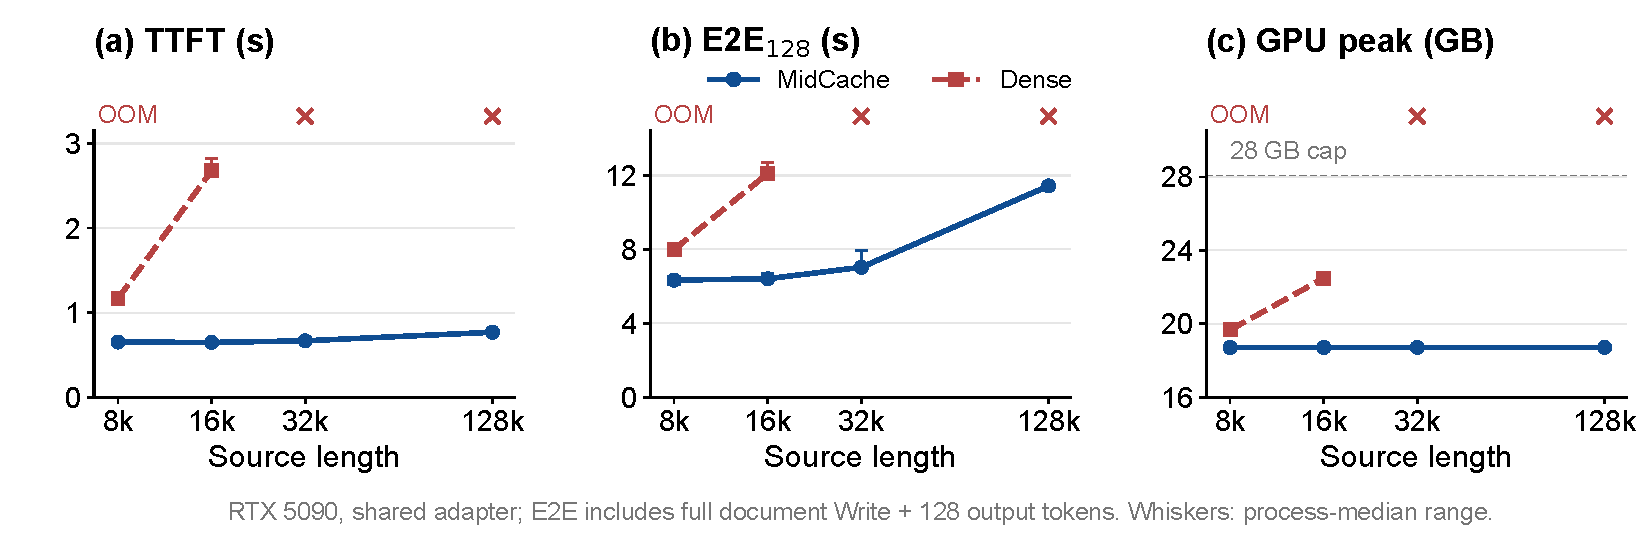
\includegraphics[width=\linewidth]{figures/source_scaling.pdf}
\caption{\textbf{Source-length scaling on RTX 5090.} These are the Table~\ref{tab:infra}(a) measurements with a shared adapter and three documents per length. Source length uses a base-two logarithmic axis. Latency markers are medians of three process medians; whiskers show their range, not a confidence interval. TTFT excludes document Write; E2E includes fresh document preparation and a fixed 128-token output. GPU values are maximum TTFT allocated peaks including weights. Red crosses above the axes mark Dense OOMs at 32k and 128k under the 28 GB allocator cap; they have no numerical ordinate. MidCache's 32k/128k measurements use a tighter 26 GB cap. Full inputs, repetition counts, and timing boundaries are specified in this appendix.}
\label{fig:source-scaling}
\end{figure}

The RTX 5090 measurements use Windows, PyTorch 2.7.1+cu128, Transformers 5.16.1, two intra-op and sixteen inter-op CPU threads, and SDPA with explicit KV-head repetition. Qwen3-8B weights remain bf16 and fully GPU resident. All local methods share the principal unmerged fp32 rank-32 suffix adapter spanning layers 12--35, with the training configuration specified in Appendix~\ref{app:protocol}. The PG-19 timing inputs differ from the benchmark questions, so these costs are not item-paired with Table~\ref{tab:accuracy}.

At each length, three saved PG19 documents supply the complete source and its next 512 tokens as the query: book indices 0/1/2 at 8k, 16k, and 32k, and 0/1/32 at 128k. Queries therefore differ across source lengths. These are fixed, unscored systems workloads. MidCache's iterative token-ID BM25 uses the first 32 query tokens, hop width two, and top-12 source-order chunks of 512 tokens. Its suffix receives 6,657 residual-state positions at $j=12$: 6,144 cached source positions, 512 query positions, and one BOS sink. Dense instead receives all 8,705, 16,897, 33,281, or 131,585 token IDs without retrieval.

\paragraph{Full-source Dense under the memory limit.}
\label{app:local-dense28}
\begin{table}[htbp]
\centering
\small
\setlength{\tabcolsep}{4pt}
\begin{tabularx}{\linewidth}{lll*{5}{>{\raggedleft\arraybackslash}X}}
\toprule
Source & Method & Phase & P1 & P2 & P3 & Peak GB & OOM\\
\midrule
8k & Dense & Prefill & 1194.4 & 1222.1 & 1159.5 & 19.66 & 0/9\\
 &  & TTFT & 1165.9 & 1231.9 & 1162.5 & 19.66 & 0/9\\
 &  & E2E$_{128}$ & 8124.3 & 7987.6 & 7643.4 & 19.66 & 0/9\\
\midrule
8k & CoMem & Prefill & 607.1 & 640.5 & 601.9 & 18.68 & 0/9\\
 &  & TTFT & 652.6 & 672.4 & 639.2 & 18.71 & 0/9\\
 &  & E2E$_{128}$ & 6537.7 & 6331.6 & 6073.1 & 18.71 & 0/9\\
\midrule
16k & Dense & Prefill & 2819.0 & 2684.8 & 2679.0 & 22.49 & 0/9\\
 &  & TTFT & 2820.0 & 2681.3 & 2680.2 & 22.49 & 0/9\\
 &  & E2E$_{128}$ & 12680.3 & 12085.8 & 12093.9 & 22.49 & 0/9\\
\midrule
16k & CoMem & Prefill & 634.3 & 606.5 & 602.8 & 18.68 & 0/9\\
 &  & TTFT & 685.2 & 647.0 & 648.0 & 18.71 & 0/9\\
 &  & E2E$_{128}$ & 6703.1 & 6407.2 & 6392.6 & 18.71 & 0/9\\
\midrule
32k & Dense & Prefill & OOM & OOM & OOM & OOM & 9/9\\
 &  & TTFT & OOM & OOM & OOM & OOM & 9/9\\
 &  & E2E$_{128}$ & OOM & OOM & OOM & OOM & 9/9\\
\midrule
128k & Dense & Prefill & OOM & OOM & OOM & OOM & 9/9\\
 &  & TTFT & OOM & OOM & OOM & OOM & 9/9\\
 &  & E2E$_{128}$ & OOM & OOM & OOM & OOM & 9/9\\
\bottomrule
\end{tabularx}
\caption{Fresh RTX 5090 measurements with the shared adapter and a 28 GB total CUDA allocator cap. Dense receives the full source plus 513 query/BOS tokens; CoMem resumes from cached $j=12$ residual states of 12 selected chunks. P1--P3 are independent process medians in milliseconds, each from three documents with one warmup and three formal repetitions per document. OOM counts failed document/process cells out of nine; repetitions stop after an OOM. Failed entries have no completed latency or peak-memory value. Peak GB is the maximum allocated memory including weights. Retained 32k/128k CoMem process results appear in the subsequent diagnostic tables.}
\label{tab:dense5090}
\end{table}

Dense uses the standard model forward with a complete KV cache and only the final vocabulary logits. There is no truncation, quantization, CPU weight/KV offload, or RoPE extension. Fused SDPA is required and the quadratic-memory math backend is disabled. A 28,000,000,000-byte process CUDA allocator cap includes weights, inputs, KV, and temporary tensors; both allocated and reserved memory remain within it. Desktop and driver-context overhead are separate from this allocator budget. Each of three fresh processes attempts every source length, document, and phase. A CUDA OOM is recorded with its error and full input shape; remaining repetitions of that failed cell are skipped. Other errors fail the worker rather than becoming OOM entries. Any failed prescribed document/process cell makes the corresponding overview entry OOM, without a latency or a selectively reported successful-subset mean.

Dense Prefill starts with the entire ID sequence on GPU and ends at first logits. TTFT starts with pretokenized CPU source/query, assembles and pins the full IDs, transfers them, and runs the same cached forward. E2E continues to 128 generated token IDs, including the first token and 127 cached decode steps; EOS does not shorten this fixed budget. Model loading, tokenization/detokenization, queues, network transport, and external I/O are excluded. Each worker checks cached greedy decoding against full recomputation before formal measurement; the short-source workers also check MidCache's cached decode against pack recomputation. Beyond-native full-source timings are not an accuracy claim.

\paragraph{MidCache preparation and request boundaries.}
At 8k and 16k, both methods are measured in the same three processes under the 28 GB cap, with shuffled method and phase order. At 32k and 128k, MidCache uses a stricter 26 GB allocator cap. The same model, adapter, and saved inputs are used within each source length. MidCache Prefill starts with GPU-ready residuals, while TTFT additionally includes BM25 construction/selection, pinned fetch, and sink/query Write. These two phases exclude document Write and decode. E2E begins with the pretokenized source/query and includes preparing a new pinned store, independently writing every source chunk, retrieval, fetch, sink/query Write, prefill, and a fixed 128-token output. It stops before store/cache teardown. Document Write is charged in full, without amortization. At 128k the residual store is 1 GiB of CPU memory, separate from GPU allocation.

Dense at every length and MidCache at 8k/16k use one warmup and three formal repetitions per successful cell: 27 formal observations per source/method/phase across three processes and three documents. MidCache Prefill and TTFT at 32k/128k use five warmups and twenty formal repetitions per document (180 observations per cell); MidCache E2E at these lengths uses one warmup and three repetitions (27 observations). Reported latencies are medians of process medians; GPU peaks are maximum allocated bytes including weights. Phases are timed independently, so small Prefill/TTFT median reversals can occur with run-to-run variation; their difference is not an isolated transfer-cost estimate. E2E is timed directly, not added from separate medians. All local inputs and generated IDs, phase boundaries, checks and raw attempts are saved.

\paragraph{Same-evidence depth diagnostics.}
\begin{table}[htbp]
\centering
\small
\setlength{\tabcolsep}{4pt}
\begin{tabular}{@{}lllrrrr@{}}
\toprule
Source & Method ($k$) & Phase & Process 1 & Process 2 & Process 3 & Peak GB\\
\midrule
32k & Replay (12) & Prefill & 835.1 & 836.3 & 835.0 & 19.01\\
32k & MidCache (12) & Prefill & 611.9 & 611.5 & 611.8 & 18.68\\
32k & Replay (12) & TTFT & 867.7 & 867.7 & 868.5 & 19.01\\
32k & MidCache (12) & TTFT & 667.5 & 666.7 & 667.6 & 18.71\\
\midrule
128k & Replay (12) & Prefill & 875.1 & 882.4 & 835.9 & 19.01\\
128k & MidCache (12) & Prefill & 638.8 & 620.3 & 616.6 & 18.68\\
128k & Replay (12) & TTFT & 972.1 & 1008.6 & 957.7 & 19.01\\
128k & MidCache (12) & TTFT & 768.6 & 796.5 & 760.1 & 18.71\\
\bottomrule
\end{tabular}
\caption{RTX 5090 same-evidence depth diagnostic, separate from full-source Dense. Each process latency is the median over three documents and twenty formal repetitions per document, in milliseconds. The MidCache main-table latency is the median of these process medians; memory is the maximum allocated peak over all 180 formal observations per source length, method, and phase. Both methods use the same top-12 selected pack of 6,657 tokens and the same principal adapter; this cost workload supplies no accuracy evidence.}
\label{tab:local-infra-processes}
\end{table}

\begin{table}[htbp]
\centering
\small
\setlength{\tabcolsep}{4pt}
\begin{tabular}{@{}llrrrrr@{}}
\toprule
Source & Method & Process 1 & Process 2 & Process 3 & E2E$_{128}$ & Peak GB\\
\midrule
32k & Raw replay & 6810.1 & 6504.1 & 7127.9 & 6810.1 & 19.01\\
32k & CoMem & 7021.3 & 7026.1 & 7938.1 & 7026.1 & 18.71\\
128k & Raw replay & 6835.7 & 6916.4 & 6684.6 & 6835.7 & 19.01\\
128k & CoMem & 11426.8 & 11491.2 & 11241.1 & 11426.8 & 18.71\\
\bottomrule
\end{tabular}
\caption{RTX 5090 same-evidence E2E diagnostic, distinct from full-source Dense, including document preparation and a fixed 128-token output. Times are milliseconds. Each process median covers three documents and three formal requests per document after one warmup; E2E is the median across three independent processes (27 requests per row). Full-request GPU peaks are separate from the Prefill/TTFT peaks in Table~\ref{tab:infra}.}
\label{tab:local-e2e}
\end{table}

The raw-replay depth measurements send the same top-12 selected tokens through all layers ($j=0$), using MidCache's adapter, evidence, order, and sink. They are depth diagnostics, separate from the full-source Dense baseline in Table~\ref{tab:infra}. Their GPU inputs remain 6,657 tokens at both source lengths. Three-process Prefill/TTFT and E2E observations use the respective repetition counts above. The E2E diagnostic includes source preparation and fixed-length generation, with a fresh full-document residual store for MidCache; it does not describe Dense on the entire source.

The H20 matched-depth and TTFT-calibration experiments do not measure GPU peaks; the RTX 5090 experiments report device-specific memory costs. Persistent-store capacity, online request peak allocation, and document-Write peak allocation remain separate quantities.

\subsection{B300 full-context and selected-pack comparison}
\label{app:b300-recheck}
\begin{table}[htbp]
\centering
\small
\setlength{\tabcolsep}{7pt}
\begin{tabular}{@{}lllrr@{}}
\toprule
Method & Adapter & Model tokens & Latency (ms) & Peak GPU (GB)\\
\midrule
\multicolumn{5}{l}{\textit{GPU-ready prefill to first logits}}\\
Dense & Off & 131,585 & 14,634.5 & 50.17\\
Dense & Shared & 131,585 & 15,919.1 & 62.03\\
Raw replay & Shared & 6,657 & 246.4 & 19.04\\
CoMem & Shared & 6,657 & 194.8 & 18.71\\
\midrule
\multicolumn{5}{l}{\textit{Selected-pack TTFT with online selection and fetch}}\\
Raw replay & Shared & 6,657 & 428.9 & 19.04\\
CoMem & Shared & 6,657 & 387.9 & 18.74\\
\bottomrule
\end{tabular}
\caption{B300 measurements on three fixed 128k-source PG19 workloads. Each latency is the median of three independent process medians, each over three documents and three formal repeats after one warmup. Peak GPU allocation is the maximum over all 27 formal repetitions per row, including weights. Only the full-context diagnostic disables LoRA; all principal comparisons share the same adapter. Source length, selected-pack length, and timer boundary are distinct.}
\label{tab:b300-recheck}
\end{table}

The B300 experiment uses the same source/query tokens, selected chunk IDs, backbone, and unmerged fp32 adapter as the local 128k supplement. One Slurm-allocated B300 reports CUDA compute capability 10.3 and 287.4 GB total device memory; its driver display name is L20D. Software is PyTorch 2.14.0+cu130, Transformers 5.16.1, and PEFT 0.20.0, with two intra-op and four inter-op CPU threads. Native GQA uses fused SDPA; the math attention backend is disabled. Model weights remain bf16 and fully GPU resident.

Dense processes BOS, the complete 131,072-token source, and the 512-token query: 131,585 input tokens. It constructs a full KV cache and projects only the final vocabulary logits. MidCache and raw replay use the same 6,657-token selected pack. All document chunks are written into CPU-pinned memory before the timer; Read begins with GPU-ready tensors. TTFT additionally includes CPU iterative BM25 (including its term-frequency construction), fetch, and sink/query Write. Neither timer includes document Write, tokenization, decode, or external I/O. Source/query inputs are unscored and unextended; these costs do not establish accuracy beyond the native position window.

The same-adapter full-context/MidCache Read ratio is $81.7\times$, but the same-pack depth-only ratio is $1.265\times$ and the selected-pack TTFT ratio is $1.105\times$. The large full-context ratio therefore combines selection with depth reuse. The stock, adapter-disabled dense diagnostic gives $75.1\times$ against MidCache. Each process checks the loaded $j=0$ reader against stock last-position logits on a 256-token input before timing.

\subsection{Write-once serving and store placement}
\begin{table}[htbp]
\centering
\small
\setlength{\tabcolsep}{4pt}
\begin{tabular}{@{}lrrrr@{}}
\toprule
Source / store & $G=1$ & $G=32$ & $G=128$ & $G=512$ \\
\midrule
32k / CPU pinned & 8.9 & 9.2 & 10.9 & 94.0 \\
32k / GPU resident & 8.4 & 7.7 & 5.5 & $\infty$ \\
128k / CPU pinned & 27.6 & 29.7 & 37.4 & 520.1 \\
128k / GPU resident & 25.8 & 26.8 & 27.2 & 164.2 \\
1M / CPU pinned & 198.2 & 266.7 & 421.3 & 302.6 \\
1M / GPU resident & 180.2 & 183.0 & 190.6 & 574.7 \\
\bottomrule
\end{tabular}
\caption{Full repeated-query break-even grid. Each cell is $Q^\star$ in queries from Equation~\ref{eq:breakeven}; $G$ is generated tokens. Fetch, Read, and decode are included. Infinite crossover denotes nonpositive measured per-query savings. Values derive from three process medians and are workload-specific.}
\label{tab:break-even}
\end{table}

The serving grid compares matched selection, examples, and packs. Per-query time includes fetch, model Read, and decode; common selection cancels from Equation~\ref{eq:breakeven}. It assumes a stable, fully prepared source store: every selected chunk is a cache hit, with no eviction or corpus update charged between queries. Thus $Q^\star$ describes reuse of that store rather than an observed application hit rate. The 32k CPU-pinned preparation is 2.253\,s, compared with 2.16\,ms for the raw-token index. Values are derived from three process medians. The large-output crossovers are sensitive to small differences in decode time and should not be interpreted as a monotonic scaling law. In particular, a finite crossover is absent in one 32k GPU-resident cell.

\begin{table}[htbp]
\centering
\small
\setlength{\tabcolsep}{4pt}
\begin{tabular}{@{}lrrrrl@{}}
\toprule
Backend & Write GB/s & Fetch ms & H2D ms & Peak QPS & Outcome \\
\midrule
GPU resident & OOM & --- & --- & --- & 128 GiB $>$ 95 GiB \\
CPU pinned & 139.6 & 0.81 & 1.41 & 941 & 235 GB host \\
Local NVMe & 2.45 & 13.42 & 0.91 & 264 & 2.18 GB host \\
Network / CEPH & 1.66 & 79.20 & 1.20 & 42 & 2.19 GB host \\
\bottomrule
\end{tabular}
\caption{Persistent-store microbenchmark at 16M tokens. The same 50.3 MB top-12 pack is fetched per query; medians use seven repetitions after two warmups. Peak QPS selects the best of 1/4/16 clients and excludes model inference and retrieval.}
\label{tab:store-tiers}
\end{table}

The storage microbenchmark uses a 16M-token residual store of 128 GiB and fetches a fixed 50.3\,MB pack per query. Medians use seven repetitions after two warmups; peak QPS is the best of 1, 4, and 16 concurrent clients. These measurements include storage and transfer only, excluding BM25 and model inference. GPU residence fits 8M tokens at 64.98\,GB peak but not 16M. Off-GPU storage preserves bounded transfer volume while adding tier-dependent latency. Its QPS is not end-to-end serving throughput.

\subsection{Model timing and full-prefill references}
\begin{table}[htbp]
\centering
\small
\setlength{\tabcolsep}{4pt}
\begin{tabular}{@{}lrrrrr@{}}
\toprule
Length & Full s & CoMem s & Ratio & Full GB & CoMem GB \\
\midrule
8k & .165 & .309 & .53 & 19.92 & 17.60 \\
16k & .356 & .441 & .81 & 24.55 & 17.67 \\
32k & .826 & .681 & 1.21 & 33.82 & 17.79 \\
64k & 2.104 & 1.200 & 1.75 & 52.34 & 18.04 \\
128k & 6.035 & 2.202 & 2.74 & 89.39 & 18.54 \\
\bottomrule
\end{tabular}
\caption{Same-adapter Write-inclusive pipeline on one B200. Ratio is full time divided by CoMem time. Full processes the entire source; CoMem includes document Write, CPU retrieval, query Write, and upper-layer Read. Index construction and external I/O are excluded. Memory is peak GPU allocation.}
\label{tab:pipeline-lengths}
\end{table}

The same-adapter B200 pipeline includes document Write, CPU retrieval, query Write, and upper-layer Read through first logits, but excludes BM25 index construction and external I/O. Software is bf16/SDPA with PyTorch 2.10 and Transformers 5.5.4, and results are medians of three. Cached decode uses 20 greedy steps.

\begin{table}[htbp]
\centering
\small
\setlength{\tabcolsep}{4pt}
\begin{tabular}{@{}lrrrrr@{}}
\toprule
Method & Native A & Single 64/128k & MK 64/128k & VT 64/128k & LoCoMo F1/acc \\
\midrule
MidCache & 97.05 & 99/100 & 91/93 & 99.0/95.8 & 9.15/23.36 \\
SnapKV & 72.33$^\dagger$ & 100/100 & 94/91 & 80.0/84.8 & 9.21/22.05 \\
PyramidKV & 72.32$^\dagger$ & 100/100 & 93/89 & 88.6/86.8 & 9.13/22.10 \\
\bottomrule
\end{tabular}
\caption{Retained-KV quality at an approximately 6,657-token budget. SnapKV/PyramidKV long-length columns use full-prompt factor-4 YaRN; MidCache reads selected evidence without YaRN. $^\dagger$Native means include left-truncated 64k/128k inputs; both compression methods score 99.96 on 8k--32k. Cohort A and lexical LoCoMo metrics are used.}
\label{tab:kv-quality}
\end{table}

\begin{table}[htbp]
\centering
\small
\setlength{\tabcolsep}{4pt}
\begin{tabular}{@{}llrrr@{}}
\toprule
Method & Length & Full prefill ms & Peak GB & Decode ms/token \\
\midrule
SnapKV & 8k & 1,213 & 18.6 & 24.7 \\
SnapKV & 32k & 6,342 & 25.7 & 24.6 \\
SnapKV & 128k & 51,520 & 54.3 & 24.7 \\
PyramidKV & 8k & 1,203 & 18.6 & 24.7 \\
PyramidKV & 32k & 6,301 & 25.7 & 26.7 \\
PyramidKV & 128k & 51,520 & 54.3 & 26.8 \\
\bottomrule
\end{tabular}
\caption{Full-prefill retained-KV timing on H20, median of three with compression and 64-token generation. These methods prefill the whole source before eviction. The hardware differs from the B200 MidCache pipeline, so no cross-table speedup is inferred.}
\label{tab:kv-timing}
\end{table}

SnapKV and PyramidKV retain approximately the same token/KV budget but must first prefill the entire prompt. Their native 15-cell RULER means include left-truncated 64k/128k inputs, whereas both reach 99.96 on 8k--32k. The full-prompt long-length columns use factor-4 YaRN. The systems table times full prefill, compression, and a 64-token decode; the displayed decode column is per-token latency. These H20 values must not be combined with the B200 MidCache times to form a cross-table speedup.

\subsection{Same-backbone chunk-KV diagnostic}
\label{app:chunkkv}
\begin{table}[htbp]
\centering
\small
\setlength{\tabcolsep}{3.2pt}
\begin{tabular}{@{}llrrrrrr@{}}
\toprule
& Suffix & \multicolumn{4}{c}{LongEval accuracy} & Qasper & Payload \\
\cmidrule(lr){3-6}
Method & adapter & 8k & 16k & 32k & Mean & F1 & KiB/token \\
\midrule
Replay & off & 85 & 83 & 85 & 84.33 & 6.98 & .008 \\
Chunk-KV & off & 73 & 75 & 71 & 73.00 & 4.88 & 144 \\
MidCache (without LoRA) & off & 0 & 0 & 0 & 0.00 & 10.45 & 8 \\
\midrule
Replay & on & 80 & 77 & 76 & 77.67 & 4.65 & .008 \\
Chunk-KV & on & 59 & 62 & 46 & 55.67 & 3.68 & 144 \\
MidCache & on & 71 & 74 & 73 & 72.67 & 11.37 & 8 \\
\bottomrule
\end{tabular}
\caption{Matched evidence and explicit adapter control: 500 samples and 3,000 predictions, with 100 examples per LongEval length and all 200 Qasper examples. Both MidCache configurations use $j=12$ and $w=0$. Each path is evaluated with the same principal suffix adapter enabled or disabled; the adapter is trained for MidCache, not separately for the other paths. Chunk-KV is a CacheBlend-style reference with the first two layers fully recomputed and a fixed 15\% context-token set recomputed above them. Payload excludes the retrieval index and request-local KV; replay stores int64 IDs. These are quality measurements, not native-system latency comparisons.}
\label{tab:chunkkv}
\end{table}

The control uses the same 500 examples as Appendix~\ref{app:overlap-confirmation}: LongEval 8k/16k/32k with 100 examples per length and all 200 Qasper questions. Replay, MidCache at $j=12,w=0$, and the chunk-KV path share token IDs, selected chunks, order, sink 151643, and output budgets. Each runs with the principal adapter enabled and disabled, yielding 3,000 saved predictions across four B300 workers. An independent CPU pass checks scores, support, and selected IDs. The adapted replay and MidCache outputs match the corresponding overlap-control predictions exactly on all 500 examples.

The chunk-KV path independently prefills every selected chunk through all 36 layers, then reindexes its post-RoPE keys to contiguous pack positions. It fully recomputes layers zero and one of the assembled pack and ranks context positions by the squared L2 deviation of both keys and values at layer one. Layer-zero projections precede contextual attention and cannot supply this signal. The largest $\lceil .15N_{\mathrm{ctx}}\rceil$ deviations define a fixed source-token set recomputed through the remaining layers; sink and query positions are always recomputed. Thus the source token--layer fraction is approximately $(2+34\times.15)/36=19.72\%$, not 15\% of total execution. Full recomputation recovers stock last-position logits and the next three decode decisions in the GPU checks. This CacheBlend-style control does not implement gradual filtering, asynchronous fetch/compute overlap, or the native cache manager \citep{cacheblend}.

Table~\ref{tab:chunkkv} shows why adapter matching and deployment choice must both be visible. Applying the MidCache-trained adapter helps its own LongEval interface (0 to 72.67), but lowers replay from 84.33 to 77.67 and chunk-KV from 73.00 to 55.67. With the adapter shared, MidCache exceeds chunk-KV by 17.00 points ($[9.67,24.33]$ paired 95\% interval). Yet its 72.67 is close to unadapted chunk-KV's 73.00, so the shared-adapter difference is not evidence of an intrinsic 17-point advantage over reusable KV. No method-specific KV adapter is trained here.

On Qasper, MidCache scores 11.37 versus 4.88 for unadapted chunk-KV and 3.68 for adapted chunk-KV; all are low under the explicit-BOS, capped plain-text protocol. The shared-adapter Qasper difference is 7.68 points ($[6.30,9.07]$). Intervals use 10,000 paired resamples: examples within each LongEval length, or source-document clusters for Qasper. Full-depth bf16 GQA KV requires $2\times36\times8\times128\times2=147{,}456$ bytes/token, versus 8,192 for the residual. This establishes an 18-fold payload ratio; the quality control does not measure a native-system latency advantage.

\paragraph{Preparation, online latency, and storage.}
\begin{table}[p]
\centering
\footnotesize
\setlength{\tabcolsep}{3pt}
\begin{tabular}{@{}llrrrrrr@{}}
\toprule
Method & Adapter & Prep. & TTFT & Online$_{128}$ & E2E$_{128}$ & Store & GPU \\
 & & (ms) & (ms) & (s) & (s) & (MiB) & (GB) \\
\midrule
\multicolumn{8}{@{}l}{\textit{LongEval 8k ($n=5$)}} \\
Replay & off & 0.4 & 651.1 & 5.432 & 5.432 & 0.06 & 18.32 \\
Chunk-KV & off & 1174.2 & 352.8 & 5.109 & 6.291 & 1152.00 & 19.46 \\
CoMem (without LoRA) & off & 329.7 & 450.4 & 4.717 & 5.049 & 64.00 & 18.02 \\
\addlinespace[2pt]
Replay & on & 0.4 & 798.2 & 6.416 & 6.416 & 0.06 & 18.89 \\
Chunk-KV & on & 1441.6 & 393.9 & 5.995 & 7.445 & 1152.00 & 19.46 \\
CoMem & on & 328.1 & 597.9 & 5.688 & 6.015 & 64.00 & 18.59 \\
\midrule
\multicolumn{8}{@{}l}{\textit{LongEval 16k ($n=5$)}} \\
Replay & off & 0.6 & 658.3 & 5.437 & 5.438 & 0.12 & 18.33 \\
Chunk-KV & off & 2377.4 & 366.1 & 5.150 & 7.505 & 2304.00 & 19.46 \\
CoMem (without LoRA) & off & 664.2 & 457.9 & 4.711 & 5.379 & 128.00 & 18.02 \\
\addlinespace[2pt]
Replay & on & 0.6 & 811.1 & 6.426 & 6.427 & 0.12 & 18.90 \\
Chunk-KV & on & 2951.1 & 403.1 & 6.363 & 9.279 & 2304.00 & 19.46 \\
CoMem & on & 666.2 & 615.1 & 5.691 & 6.359 & 128.00 & 18.59 \\
\midrule
\multicolumn{8}{@{}l}{\textit{LongEval 32k ($n=5$)}} \\
Replay & off & 1.1 & 652.6 & 5.391 & 5.393 & 0.25 & 18.34 \\
Chunk-KV & off & 4647.1 & 364.4 & 5.094 & 9.739 & 4608.00 & 19.49 \\
CoMem (without LoRA) & off & 1311.2 & 457.0 & 4.703 & 6.023 & 256.00 & 18.04 \\
\addlinespace[2pt]
Replay & on & 1.1 & 803.7 & 6.399 & 6.400 & 0.25 & 18.92 \\
Chunk-KV & on & 5708.5 & 399.9 & 5.973 & 11.694 & 4608.00 & 19.49 \\
CoMem & on & 1319.2 & 613.2 & 5.685 & 7.012 & 256.00 & 18.62 \\
\midrule
\multicolumn{8}{@{}l}{\textit{Qasper ($n=5$)}} \\
Replay & off & 0.3 & 401.7 & 4.246 & 4.246 & 0.03 & 17.85 \\
Chunk-KV & off & 519.2 & 267.7 & 4.084 & 4.603 & 504.00 & 18.66 \\
CoMem (without LoRA) & off & 145.4 & 297.0 & 3.945 & 4.096 & 28.00 & 17.65 \\
\addlinespace[2pt]
Replay & on & 0.3 & 497.2 & 5.257 & 5.257 & 0.03 & 18.26 \\
Chunk-KV & on & 631.4 & 310.9 & 5.155 & 5.782 & 504.00 & 18.66 \\
CoMem & on & 146.5 & 389.9 & 5.190 & 5.334 & 28.00 & 18.06 \\
\bottomrule
\end{tabular}
\caption{Matched evidence costs on RTX 5090: 1,080 formal measurements over 20 prespecified examples, six method--adapter settings, three fresh processes, and three repetitions. Each cell reports the median of three process medians; each process median pools five examples and three repetitions. Preparation constructs a fresh whole-document pinned-CPU store. TTFT and Online start after preparation, include selection and fetch, and end at the first and 128th generated token, respectively. E2E is measured directly from preparation through token 128. Store is the median persistent payload, separate from peak GPU allocation including weights; all attempts fit the 28 GB allocator cap. CoMem uses $j=12,w=0$; replay processes the same selected evidence, not the full source. Chunk-KV is a synchronous CacheBlend-style reference. The 500-example quality evaluation is reported separately in Table~\ref{tab:chunkkv}.}
\label{tab:chunkkv-cost}
\end{table}

Table~\ref{tab:chunkkv-cost} uses the first five prespecified examples per task/length, the local software configuration above, and a 28 GB allocator cap. All 1,080 formal trials and 360 warmups complete, with method--adapter order shuffled in each process. Full-recomputation and query-placeholder checks pass: recomputing every query position makes zero-initialized query KV equivalent to independently cached query states at first logits. Generated IDs match across repetitions and processes within each setting.

Each trial freshly prepares the entire pretokenized document in pinned CPU memory: int64 IDs for replay, bf16 residuals for MidCache, or bf16 all-layer KV for chunk-KV. Preparation includes partitioning, pinning, and document Write. TTFT then includes BM25 construction/selection, transfer, sink/query handling, and inference through token one. Online continues to token 128 regardless of EOS; E2E directly times preparation through token 128, before teardown. Loading, tokenization/detokenization, external I/O, and scoring are excluded. Payload excludes selector metadata and transient raw IDs; GPU peaks include weights and preparation/inference allocations. Qasper lengths vary, so payload is a median. Separate medians need not add.

Chunk-KV has lower TTFT than MidCache in every cell under both adapter conditions, but needs more storage and preparation. At 32k with the shared adapter, chunk-KV versus MidCache takes 399.9 versus 613.2\,ms TTFT, 5.708 versus 1.319\,s preparation, and 11.694 versus 7.012\,s E2E. Process-median TTFT ranges are 397.4--412.8 and 608.2--640.0\,ms; these are descriptive, not confidence intervals. Persistent payload is 4,608 versus 256 MiB, while peak GPU allocation is 19.49 versus 18.62 GB: the 18-fold storage ratio does not describe GPU peaks. MidCache also has higher cold-request E2E than shared-adapter replay at 32k (7.012 versus 6.400\,s). These subset timings do not establish native CacheBlend performance or accuracy rankings.

\subsection{Latency-calibrated budget comparison}
\label{app:equal}
\begin{table}[htbp]
\centering
\small
\setlength{\tabcolsep}{4pt}
\begin{tabular}{@{}lcccc@{}}
\toprule
Replay selector & Replay / MidCache & Delta & Hierarchical CI & LOCO range \\
\midrule
Iterative BM25 & 64.78 / 53.22 & -11.56 & [-18.67, -5.11] & [-13.13, -9.50] \\
Frozen BGE & 54.22 / 53.22 & -1.00 & [-10.67, 8.33] & [-3.50, 1.75] \\
\bottomrule
\end{tabular}
\caption{Comparison at latency-calibrated maximum chunk budgets: ten for replay and twelve for MidCache. Per-cell latency on the quality mixture is unreported. Delta is MidCache minus replay, in points, averaged equally over nine cells. Hierarchical intervals are 95\%; LOCO denotes leave-one-cell-out sensitivity. Only the replay selector changes in the BGE diagnostic.}
\label{tab:equal-latency}
\end{table}

\begin{table}[htbp]
\centering
\small
\setlength{\tabcolsep}{4pt}
\begin{tabular}{@{}lcc@{}}
\toprule
Cell & BM25 delta & BGE delta \\
\midrule
BABILong qa1 / 4k & -6 & -5 \\
BABILong qa1 / 16k & -17 & -21 \\
BABILong qa2 / 4k & -3 & 0 \\
BABILong qa2 / 16k & -10 & -23 \\
LongEval / 8k & -26 & 0 \\
LongEval / 16k & -28 & 16 \\
RULER multikey / 8k & -6 & 1 \\
RULER multikey / 16k & -9 & 19 \\
LoCoMo / first 100 & 1 & 4 \\
\midrule
Fixed-cell 95\% CI & [-14.33, -8.78] & [-4.56, 2.56] \\
Pooled-IID 95\% CI & [-14.44, -8.67] & [-4.67, 2.67] \\
\bottomrule
\end{tabular}
\caption{Cell-specific quality deltas at the latency-calibrated chunk budgets and sensitivity intervals. Each cell has 100 paired examples; LoCoMo contains only one conversation. Positive deltas favor MidCache. The pooled-IID interval is reported only as sensitivity, not the task-mixture inference.}
\label{tab:equal-cells}
\end{table}

Quality is the equal-weight mean of nine 100-example cells: BABILong qa1 and qa2 at 4k/16k, LongEval at 8k/16k, RULER multikey at 8k/16k, and the first 100 LoCoMo questions. The latter are all from conversation zero. They cannot support a conversation-cluster bootstrap. Generation is greedy and no-chat: BABILong allows 20 tokens with official scoring, LongEval 16 with numeric exact match, RULER 48 with official string matching, and LoCoMo 48 with the local substring/F1-threshold or abstention diagnostic rather than the headline GPT-4o judge.

Calibration uses only TTFT on three reserved RULER multikey 32k documents, indices 900--902, disjoint from quality indices 0--99. The experiment seed is 42 and \texttt{PYTHONHASHSEED=0}. It considers maximum budgets $k\in\{2,4,6,8,10,12,14,16,20,24\}$ and selects a replay budget within a declared $\pm5\%$ band of MidCache's budget-12 anchor. Selectors may under-fill. One H20 uses bf16/SDPA, three independent processes per budget, five warmups, and 20 repetitions. TTFT includes online selection, raw/residual fetch, sink/query Write, and prefill to first logits; it excludes decode, document Write, and index construction.

BM25 replay at budget ten takes 703.7\,ms, against MidCache at 698.3\,ms with GPU storage or 699.8\,ms with CPU storage. BGE replay takes 697.8\,ms, against MidCache at 700.5/702.2\,ms. The BGE condition changes only replay's retriever; it is not a matched-evidence depth control.

Statistical analyses use 100,000 paired resamples with base seed 20260804. Fixed-cell bootstrapping keeps all cells and resamples 100 pairs within each. Hierarchical bootstrapping resamples nine cell labels, then 100 pairs within each selected occurrence. Leave-one-cell-out ranges assess sensitivity to the mixture. Pooled-IID intervals are reported as sensitivity only; the task-mixture inference uses the hierarchical intervals.

\subsection{Store scale and coverage limits}
\begin{table}[htbp]
\centering
\small
\setlength{\tabcolsep}{4pt}
\begin{tabular}{@{}lcccc@{}}
\toprule
Store & NIAH / VT recall & NIAH / VT score & Read tokens & BM25 ms \\
\midrule
128k & 1.00 / 1.00 & 100 / 18 & 6,211 / 6,463 & 80 / 20 \\
256k & 1.00 / 1.00 & 100 / 34 & 6,209 / 6,463 & 164 / 39 \\
512k & 1.00 / 1.00 & 100 / 40 & 6,209 / 6,464 & 328 / 81 \\
1M & 1.00 / 1.00 & 100 / 54 & 6,209 / 6,463 & 697 / 170 \\
2M & 1.00 / 1.00 & 90 / 38 & 6,211 / 6,463 & 1,407 / 357 \\
4M & 1.00 / 1.00 & 100 / 34 & 6,208 / 6,463 & 2,852 / 725 \\
\bottomrule
\end{tabular}
\caption{Fixed top-12 store scaling. Slash-separated entries are single-evidence NIAH / five-link variable tracking. Evidence recall uses $n=20$ and generated scores $n=10$. Model Read remains bounded while retrieval latency grows; perfect recall does not guarantee correct reasoning.}
\label{tab:store-scale}
\end{table}

With fixed top-12, the reader sees about 6.2--6.5k tokens as the store grows from 128k to 4M. Evidence recall uses 20 examples and generation uses ten. Perfect evidence recall does not guarantee successful variable tracking: the generated scores remain noisy. At 128k, increasing the required VT evidence count from 12 to 16, 24, and 32 reduces recall from 1 to 0.75, 0.50, and 0.375, matching $\min(1,12/E)$ when $E$ evidence chunks are required. Co-keyed multivalue evidence has recall 0.62 even at $E=8$. A common-word-frequency task scores zero as coverage drops from 4.5\% at 128k to 1.2\% at 512k. Bounded selected reads do not provide general global aggregation.

\FloatBarrier
\section{Statistical Analysis and Data Qualifications}
\label{app:stats}
\subsection{LoCoMo judging and uncertainty}
GPT-4o scores 1,540 answerable items in categories 1--4; the 446 category-5 items use the local abstention rule. Category sizes are 282, 321, 96, 841, and 446. The full-set Judge is over all 1,986 examples. Category-5 success includes an empty answer or a match to the refusal rule, whereas empty answers on answerable items are failures.

The judge run is dated July 22, 2026 and uses an OpenAI-compatible endpoint named \texttt{gpt-4o}, seed one, with no client-set temperature or top-$p$. The endpoint has no dated model snapshot. Its prompt supplies question, gold answer, and prediction, accepts semantic equivalence including equivalent dates, rejects contradictions and omissions, and requests \texttt{CORRECT} or \texttt{WRONG}. Gold alternatives are joined with ``OR.'' Parsing expects the label at the start, with a fallback substring vote. Requests retry four times with exponential backoff; failures or unparsable results default to wrong. The records contain example IDs and parsed decisions.

On the common answerable items, CoMem scores 48.64 and KV-Direct 43.83. Their paired $+4.81$-point difference has a 95\% item-bootstrap interval of $[2.34,7.34]$ using 10,000 resamples and seed 1234. Resampling the ten conversations instead gives $[1.27,8.32]$; eight of ten observed conversation differences favor CoMem. The cluster interval addresses dependence but does not create additional independent conversations, and its tail fraction is not reported as a calibrated hypothesis-test $p$ value.

An independent July 26, 2026 audit applies DeepSeek-V3 to a stratified 200-item paired subset. Agreement with GPT-4o is 0.81, with $\kappa=0.626$. GPT-4o scores CoMem/KV-Direct at 36.5/32.5 and DeepSeek-V3 at 56.0/49.0. The ordering persists on this subset, although absolute calibration differs.

Descriptive per-method intervals use 1,000 item-bootstrap resamples with seed 1234: full-set Judge is $[36.20,40.58]$ for CoMem and $[32.48,36.71]$ for KV-Direct; answerable-item Judge is $[46.04,50.98]$ and $[41.23,46.30]$; F1 is $[8.60,9.72]$ and $[8.51,9.61]$. These unpaired intervals do not replace the paired cluster comparison. The six-length LongEval mean has 95\% interval $[69.33,76.33]$; the main table instead uses the five-length mean of 69.0.

\subsection{Prompt and training-run sensitivity}
\begin{table}[htbp]
\centering
\small
\setlength{\tabcolsep}{4pt}
\begin{tabular}{@{}lrrrrr@{}}
\toprule
Metric & Seed 42 & Seed 1 & Seed 2 & Mean & SD \\
\midrule
RULER 9-cell macro & 98.80 & 99.42 & 98.76 & 98.99 & .37 \\
BABILong 9-cell macro & 38.44 & 40.33 & 41.44 & 40.07 & 1.52 \\
RULER MK 3-length mean & 96.67 & 98.67 & 96.67 & 97.33 & 1.15 \\
BABILong qa5 3-length mean & 66.00 & 69.33 & 71.00 & 68.78 & 2.55 \\
\bottomrule
\end{tabular}
\caption{Seed-plus-effective-batch sensitivity. Seed 42 uses effective batch eight; seeds one and two use batch three with matched examples seen. These settings differ from the principal batch-one recipe. RULER uses three tasks at 32k/64k/128k, $n=50$ per cell; BABILong uses three tasks at 4k/16k/32k, $n=100$. SD is sample SD of three run-level macros. This is not pure seed variance or the principal 15-cell RULER cohort.}
\label{tab:run-robustness}
\end{table}

Native chat formatting changes CoMem's LoCoMo Judge from 38.27 to 37.76 and KV-Direct's from 34.59 to 38.22, reversing their order. Lexical metrics change more strongly: CoMem F1/substring accuracy goes from 9.15/23.36 to 19.51/28.65, and KV-Direct F1 goes from 9.02 to 40.06. The no-chat semantic comparison is therefore protocol-specific. No matched native-chat evaluation is available for MemoryLLM, so no corresponding sensitivity conclusion is drawn.

The batch-size sensitivity experiment uses effective batches eight, three, and three with matched examples seen. It jointly assesses seed and optimization-noise variation, rather than pure seed variance or variation of the principal batch-one training recipe. Across 18 reduced-support RULER and BABILong cells, median cell-wise SD is 1.34 points and the maximum is 4.36. These are not the exact 15-cell Cohort-B headline, and no multi-run LoCoMo or LongEval headline is available.

\subsection{Training-corpus overlap}
\label{app:clean-longbench}
The PG-19 overlap audit uses normalized 13-gram containment sketches. On InfiniteBench long-book support, a threshold of 0.8 flags 24/86 books and 163/580 records. Containment is bimodal: 31 books are below 0.10, none lies in 0.18--0.60, and 54 reach at least 0.60. A cut in 0.20--0.60 therefore flags 54 books and 387 records; anonymized character names make the 0.8 count conservative. The available results lack predictions for the strict clean subset of 113 QA and 76 choice records. That benchmark's book-quality comparison is excluded.

The natural-task audit finds no flagged LoCoMo overlap; LongEval is synthetic. For LongBench, the strict criterion is normalized 13-gram sketch containment below .10 against the complete PG-19 training split, a conservative reference relative to the 64-book adapter corpus. It removes 96/200 NarrativeQA examples and one of 200 2WikiMQA examples. The other four tasks are unchanged, leaving 1,053 of 1,150 examples. Dataset IDs and row indices independently confirm filter membership.

\begin{table}[htbp]
\centering
\small
\setlength{\tabcolsep}{5pt}
\begin{tabular}{@{}lrrrrrr@{}}
\toprule
& \multicolumn{2}{c}{NarrativeQA} & \multicolumn{2}{c}{2WikiMQA} & \multicolumn{2}{c}{Six-task macro} \\
\cmidrule(lr){2-3}\cmidrule(lr){4-5}\cmidrule(l){6-7}
Method & Full & Clean & Full & Clean & Full & Clean \\
\midrule
Replay $j=0$ & 3.81 & 3.99 & 12.34 & 12.31 & 12.18 & 12.21 \\
MidCache & 4.03 & 4.32 & 10.72 & 10.69 & 12.01 & 12.05 \\
MidCache (without LoRA) & 3.87 & 4.14 & 9.65 & 9.62 & 9.86 & 9.90 \\
\bottomrule
\end{tabular}
\caption{Full and strict-clean LongBench F1 from the same per-method predictions. NarrativeQA retains 104/200 examples and 2WikiMQA retains 199/200; the other four datasets are unchanged, giving 1,053/1,150 examples. The macro weights all six datasets equally in both columns. Both MidCache configurations use $j=12$; replay has no adapter. Full-set values are the corresponding results in Table~\ref{tab:longbench-detail}. Filtering uses source-document containment below .10 against the full PG-19 training split and is independent of method outputs.}
\label{tab:clean-longbench}
\end{table}

Table~\ref{tab:clean-longbench} re-scores the same full-set predictions used by the two CoMem configurations and unadapted replay. All three share input IDs, selected chunk IDs and order, generation limits, and the last-chunk query boundary. The full-set macro F1 is 12.01 for CoMem, 9.86 without LoRA, and 12.18 for replay; the clean-set values are 12.05, 9.90, and 12.21. The macro retains equal weights for all six tasks after filtering. The change in full versus clean score reflects a changed population and is not a causal estimate of contamination's effect.

CoMem's paired clean-set gain over its no-LoRA variant is 2.15 points (95\% interval $[1.57,2.72]$); its difference from replay is $-.15$ ($[-.71,.38]$). Full-set intervals are $[1.57,2.71]$ and $[-.67,.32]$, respectively. We use 10,000 paired source-document-cluster resamples within each dataset, recompute its item mean, then average the six task means (seed 20260913). The filtering preserves the adaptation gain and leaves the small replay difference unresolved. Other external baselines lack clean-set predictions here. Near-verbatim filtering cannot exclude semantic paraphrase or exposure through unknown backbone-pretraining corpora.

\FloatBarrier
\section{Limitations}
\label{app:limitations}
\paragraph{Quality and generality.}
The main evidence concerns one Qwen3-8B checkpoint, English benchmarks, lexical retrieval, and one flagship adapter. Raw replay is stronger on the matched depth test and the same-selector mixture at latency-calibrated chunk budgets; LongEval shows a large representation cost, and LoCoMo's full-context ordering reverses under chat formatting. The diagnostic BGE difference is unresolved. Broader model sweeps test portability rather than matched replication, and the additional training runs confound seed with effective batch size. The probe results concern accessibility to a readout, not the causal location of understanding.

\paragraph{Scope of repair.}
The context--position control broadens query and decode visibility as well as document states, so it does not isolate document-cache fidelity. The multikey overlap gain does not generalize to the independent LongEval/Qasper evaluation; the latter uses capped plain-text generation and yields low QA scores. The separate trained writer still lacks natural-task validation. An oracle computed afresh on the full pack is not a reusable solution. Other error sources may dominate on tasks requiring broad coverage, long chains, or low-overlap retrieval.

\paragraph{Serving assumptions.}
The workload assumes repeated queries over stable corpora with open-weight models. Residual storage is linear and substantially larger than token IDs; indexing and lookup grow with the store. Changing the tokenizer, model weights, split, or lower-layer computation may require rewriting states. Overlap can propagate invalidation into a neighboring chunk. Timing depends on hardware, kernels, batch size, storage tier, and generation length. The reported request measurements are single-query medians, without concurrent model throughput or p95/p99 tails; large-output crossovers can be unstable. Quantization, eviction, update contention, and multi-tenancy are not evaluated.

\paragraph{Comparators and reproducibility.}
The CacheBlend-style controls match evidence and both adapter settings, but use two full bootstrap layers and a fixed repair set, not the native serving system. Timings cover 20 examples with synchronous fetch/recomputation; the shared MidCache adapter is not KV-specific adaptation. Other PIC and learned modular-cache systems lack matched backbone/hardware comparisons. Full-context, retained-KV, same-pack replay, and store-ready measurements answer different questions. The undated GPT-4o endpoint and ten LoCoMo conversations limit reproducibility and population inference. LongBench clean-subset analysis covers three methods and near-verbatim PG-19 overlap, leaving backbone-pretraining exposure unknown. Formatted-example quality tests differ from source/query-separated serving. Long-form generation, code, multilingual, multimodal, and continually updated memory remain open.

\end{document}
